\documentclass[]{beamer}

\usetheme[block=fill]{metropolis}

%\usepackage{beamerthemesplit}
\usepackage{tabularx}
\usepackage{epstopdf}
\usepackage{amsmath}
\usepackage{tipa}
\usepackage{mathptmx}
\usepackage[11pt]{moresize}
\usepackage{tikz}
\usepackage{drawstack}
\usepackage{booktabs}
\usepackage{multirow}

\usetikzlibrary{matrix}
\usetikzlibrary{positioning}
\usetikzlibrary{shapes}
\tikzset{%
  stack/.style={%
    rectangle split,%
    draw,%
    text width=10em,%
    minimum width=10.1em,%
    anchor=west}
}

% solarized color scheme
\definecolor{base03}{HTML}{002B36}
\definecolor{base02}{HTML}{073642}
\definecolor{base01}{HTML}{586E75}
\definecolor{base00}{HTML}{657B83}
\definecolor{base0}{HTML}{839496}
\definecolor{base1}{HTML}{93A1A1}
\definecolor{base2}{HTML}{EEE8D5}
\definecolor{base3}{HTML}{FDF6E3}
\definecolor{yellow}{HTML}{B58900}
\definecolor{orange}{HTML}{CB4B16}
\definecolor{red}{HTML}{DC322F}
\definecolor{magenta}{HTML}{D33682}
\definecolor{violet}{HTML}{6C71C4}
\definecolor{blue}{HTML}{268BD2}
\definecolor{cyan}{HTML}{2AA198}
\definecolor{green}{HTML}{859900}
\definecolor{lightorange}{RGB}{255,200,150} % Adjust the RGB values as needed
\definecolor{lightblue}{RGB}{173,216,230}   % Adjust the RGB values as needed

\usepackage{listings}
\lstset{%
  showspaces=false,
  showtabs=false,
  breaklines=true,
  belowskip=10pt,
  aboveskip=10pt,
  abovecaptionskip=0pt,
  sensitive=true,
  backgroundcolor=\color{base3},
  keywordstyle=\color{cyan},
  commentstyle=\color{base1},
  stringstyle=\color{blue},
  numberstyle=\color{violet},
  showstringspaces=false,
  breakatwhitespace=true,
  basicstyle=\ttfamily\scriptsize,
  %lineskip={-1.75pt},
  columns=fullflexible,
  frame=tb
}

\makeatletter

\def\hlinewd#1{%
  \noalign{\ifnum0=`}\fi\hrule \@height #1 %
  \futurelet\reserved@a\@xhline}
\makeatother

\definecolor{pureyellow}{HTML}{FFFF00}

\newcommand*{\yellowemph}[1]{%
  \tikz\node[rectangle, fill=pureyellow, rounded corners, inner sep=0.3mm]{#1};%
}

\newenvironment{changemargin}[2]{%
  \begin{list}{}{%
      \setlength{\topsep}{0pt}%
      \setlength{\leftmargin}{#1}%
      \setlength{\rightmargin}{#2}%
      \setlength{\listparindent}{\parindent}%
      \setlength{\itemindent}{\parindent}%
      \setlength{\parsep}{\parskip}%
    }%
  \item[]}{\end{list}}

\newcommand{\tab}{\hspace*{2em}}
\newcommand*\oldmacro{}%
\let\oldmacro\insertshorttitle%
\renewcommand*\insertshorttitle{%
  \oldmacro\hfill%
  \insertframenumber\,/\,\inserttotalframenumber}
\title{x86 Crash Course}
\subtitle{With a focus on Linux and a glance to x86\_64}
\author[NECSTLab]{Mario Polino, Armando Bellante, Lorenzo Binosi}
\institute{DEIB, Politecnico di Milano}
\date{\today}

\begin{document}

\begin{frame}
	\titlepage
\end{frame}

% \begin{frame}{Credits --- contributors as of \today}
% 	\begin{itemize}
%   		\item Main contributor: Andrea Mambretti (wrote the first version)
%   		\item Mario Polino
% 		\item Marcello Pogliani
%   		\item Stefano Zanero
%   		\item Federico Maggi
%   	\end{itemize}
% \end{frame}

%\section{Crash course on x86 Assembly}

\begin{frame}
	\frametitle{How to Read the Matrix!}
  \hspace*{-11mm}
  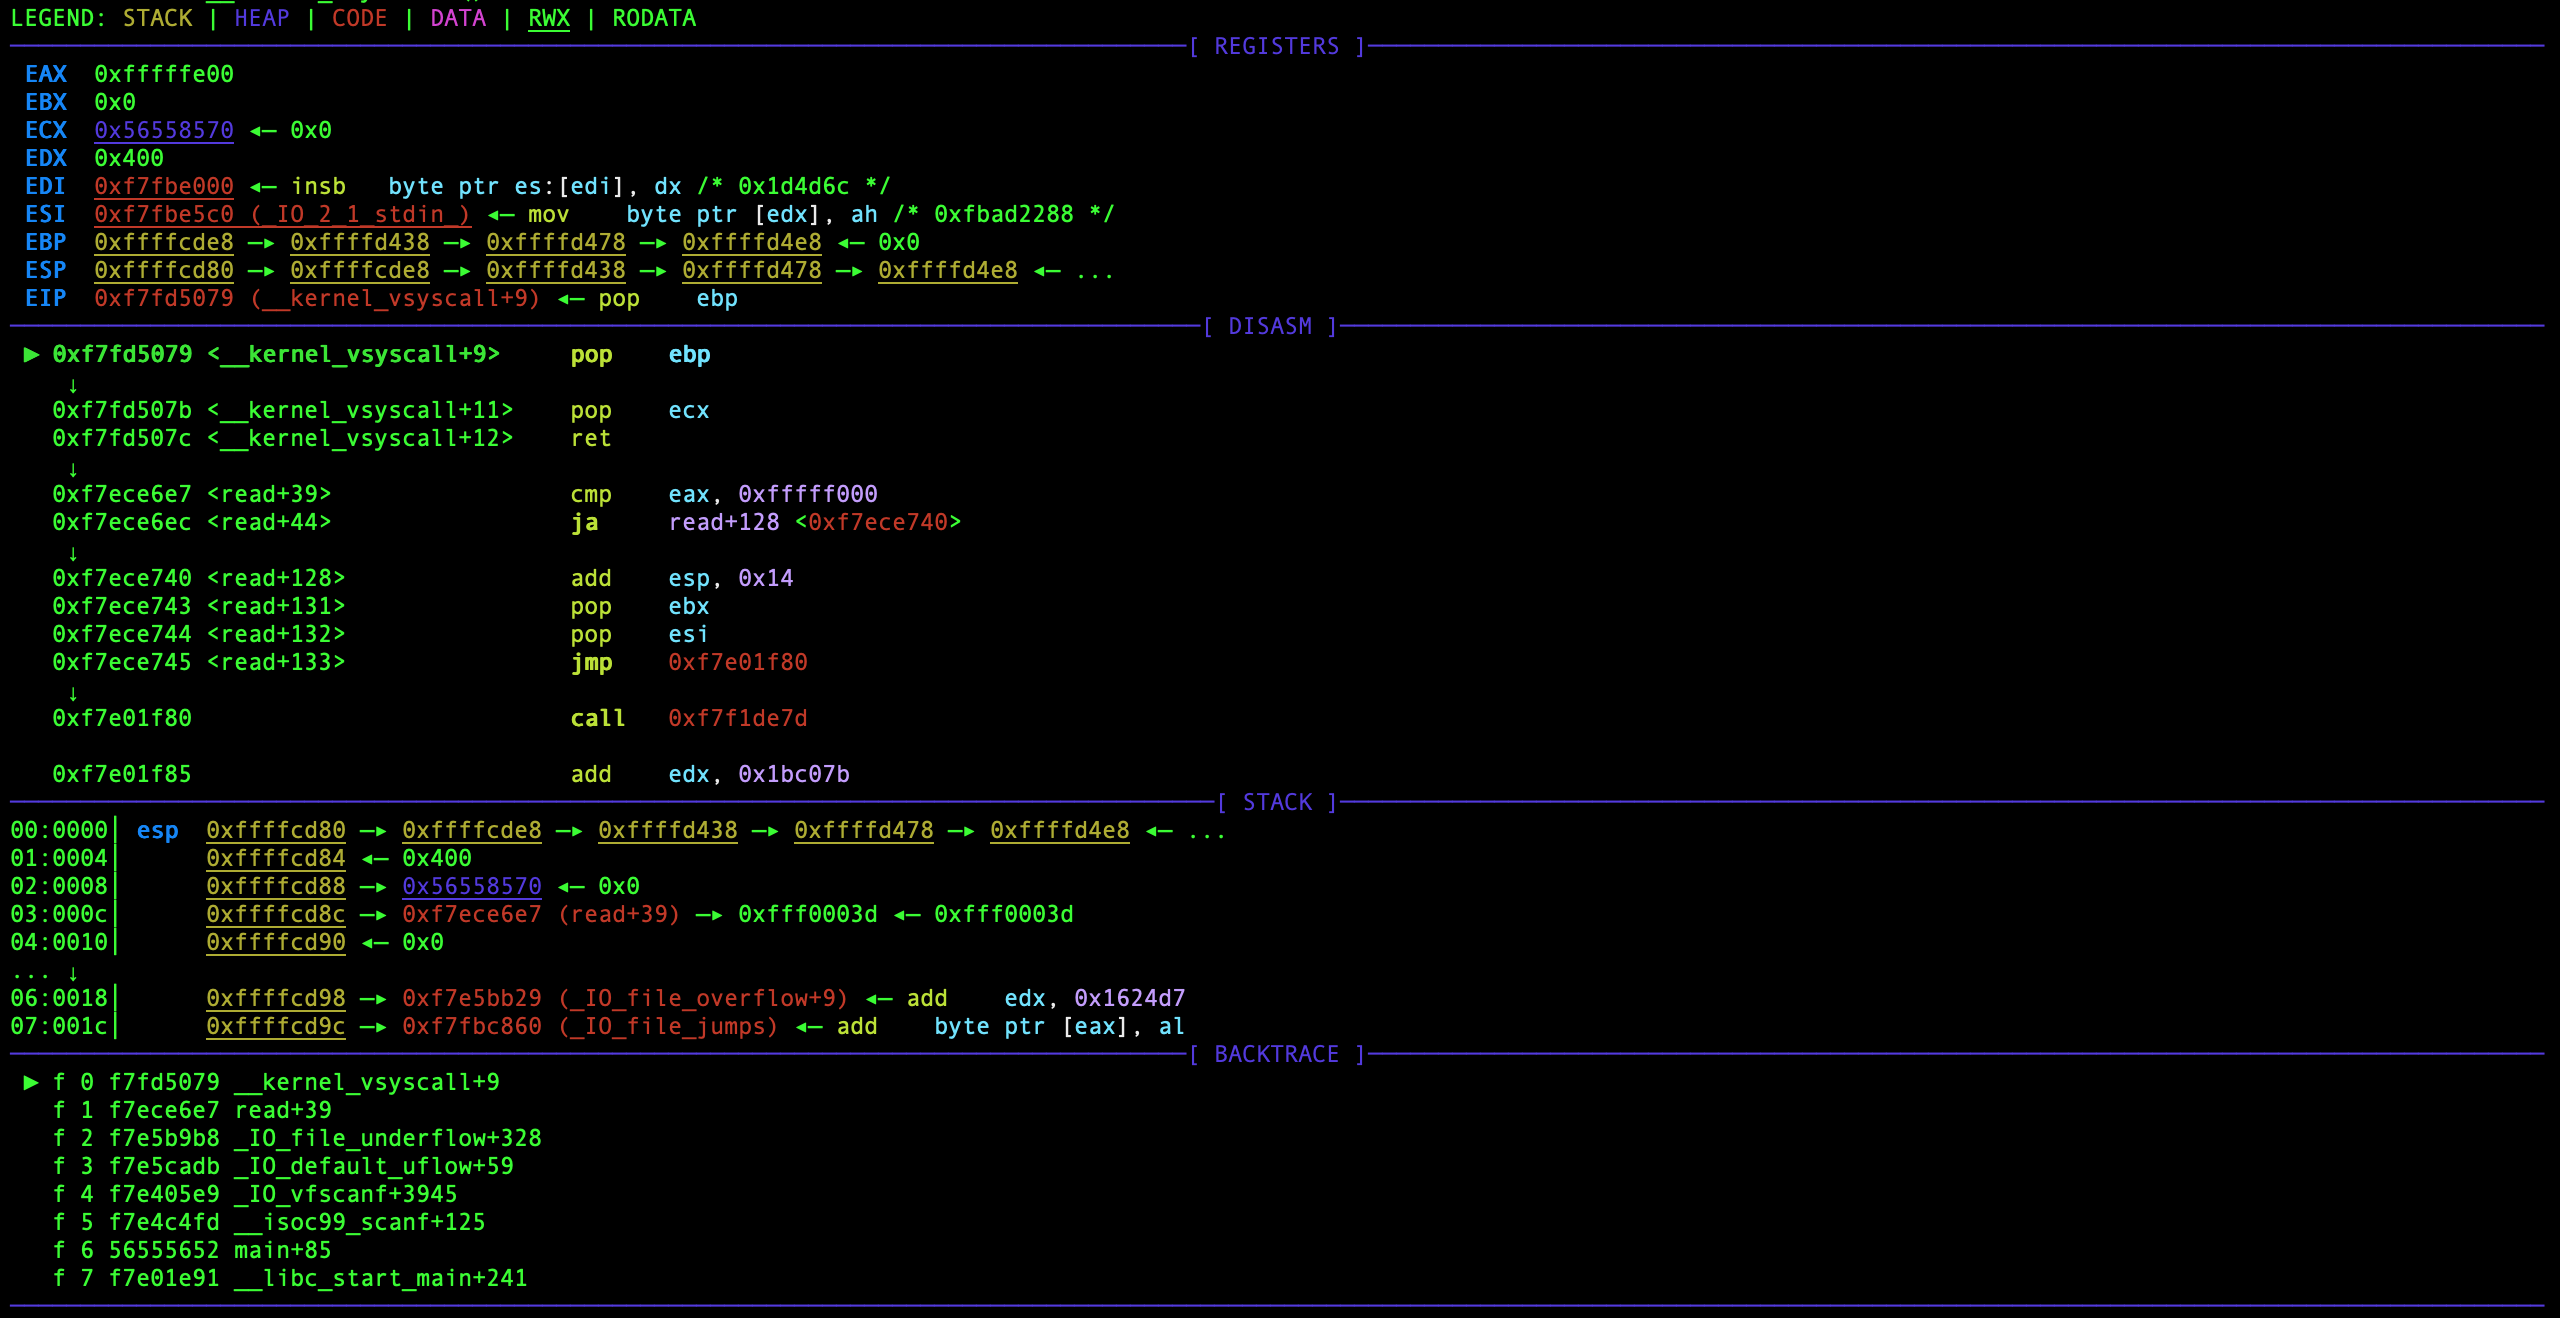
\includegraphics[width=\paperwidth]{./images/pwndbg.png}
\end{frame}
\begin{frame}
  \frametitle{Outline}
  \tableofcontents
\end{frame}

\section{The x86 Architecture}
\subsection{Overview on the common 32-bit Intel Architecture (IA)}

\begin{frame}
	\frametitle{Instruction Set Architecture (ISA)}
	\begin{itemize}
	\item ``Logical'' specification of a computer architecture
	\item Concerned with programming concepts
	\begin{itemize}
		\item instructions, registers, interrupts, memory architecture, \dots
	\end{itemize}
	\item May differ (widely) from the actual microarchitecture
	\item Examples:
		\begin{itemize}
			\item x86 (IA-32 and x86\_64)
			\item ARM (mobile devices)
			\item MIPS (embedded devices, e.g.,~consumer routers)
			\item AVR, SPARC, Power, RISC V, \dots
		\end{itemize}
	\end{itemize}
\end{frame}

\begin{frame}{The x86 ISA}
\begin{itemize}
	\item Born in 1978, 16-bit ISA (Intel 8086)
	\item Evolved to a 32-bit ISA (1985, Intel 80386)
	\item Evolved to a 64-bit ISA (2003, AMD Opteron)
	\item CISC design (e.g.,~string operations)
	\item Many legacy features (e.g,~segmentation)
	\item We'll see the basics of the ``core'' ISA
		\begin{itemize}
			\item There is also the floating point unit, processor-specific features, and extensions such as SIMD (MMX, SSE, SSE2) with their own instructions and registers\footnote{Complete reference: Intel Software Developer's Manual, about 5,000 pages (\url{https://software.intel.com/en-us/articles/intel-sdm})}
		\end{itemize}
\end{itemize}
\end{frame}

\begin{frame}
  \frametitle{Von Neumann Architecture}
  %https://docs.google.com/drawings/d/1dDiokZZ4ba9V6rM9EnOCCIvbmxemN7DxXvL0ipsYPnE/edit?usp=sharing
  \begin{figure}
      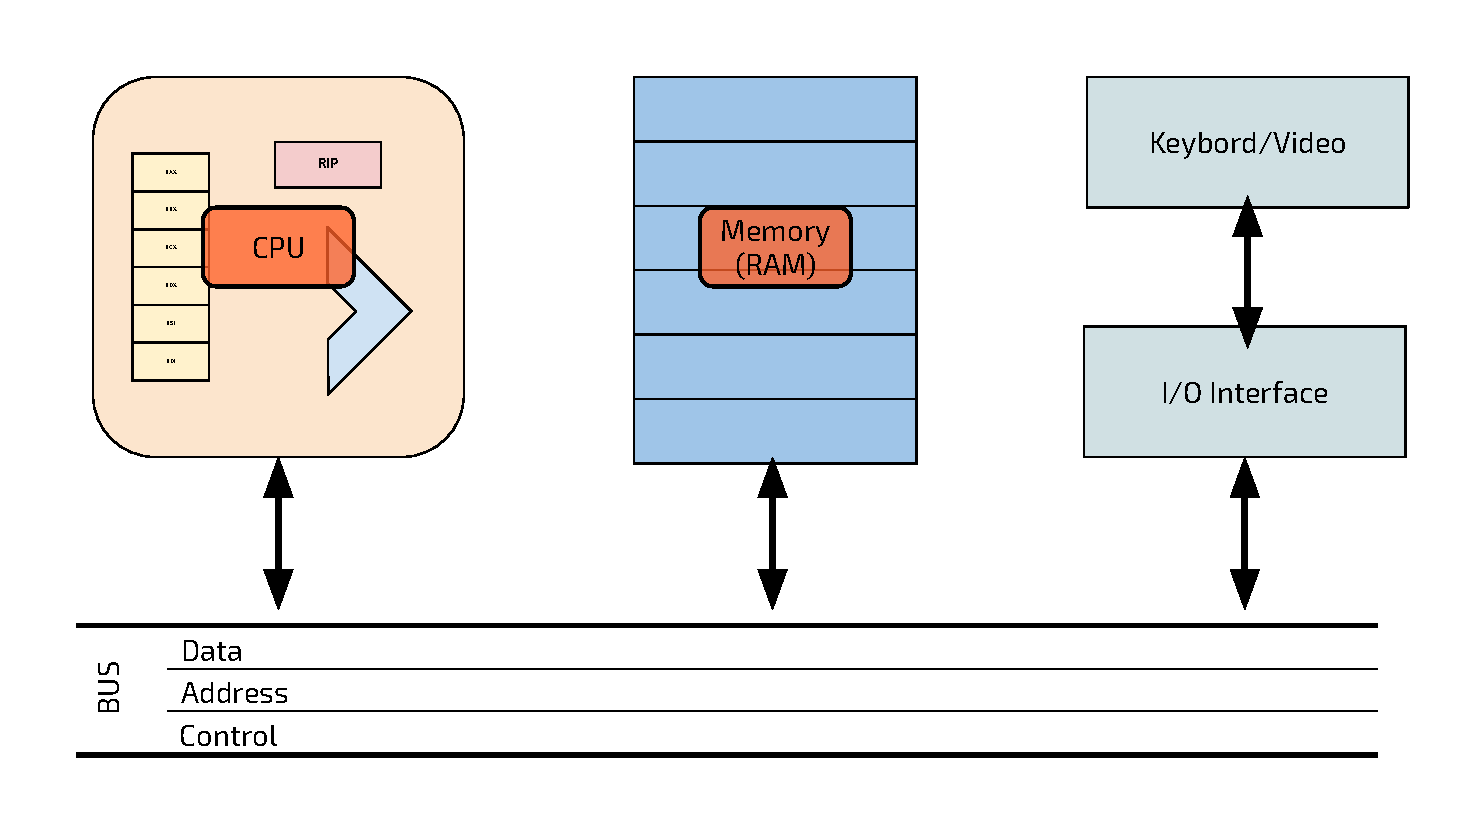
\includegraphics[height=2.3in]{images/Von-Neumann-architecture.pdf}
    \end{figure}
\end{frame}

\begin{frame}
  \frametitle{Memory}
  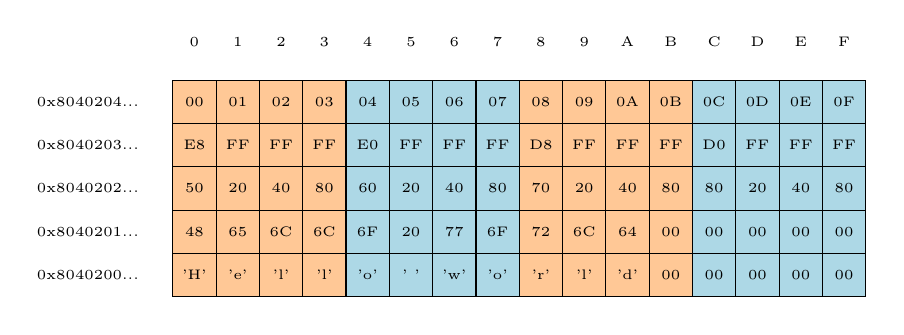
\begin{tikzpicture}[font=\tiny]
    % Draw the memory layout
    \matrix[matrix of nodes,
            ampersand replacement=\&,
            row sep=-\pgflinewidth,
            column sep=-\pgflinewidth,
            nodes={draw, minimum size=5.5mm, anchor=center, font=\tiny},
            column 1/.style={nodes={fill=lightorange}},
            column 2/.style={nodes={fill=lightorange}},
            column 3/.style={nodes={fill=lightorange}},
            column 4/.style={nodes={fill=lightorange}},
            column 5/.style={nodes={fill=lightblue}},
            column 6/.style={nodes={fill=lightblue}},
            column 7/.style={nodes={fill=lightblue}},
            column 8/.style={nodes={fill=lightblue}},
            column 9/.style={nodes={fill=lightorange}},
            column 10/.style={nodes={fill=lightorange}},
            column 11/.style={nodes={fill=lightorange}},
            column 12/.style={nodes={fill=lightorange}},
            column 13/.style={nodes={fill=lightblue}},
            column 14/.style={nodes={fill=lightblue}},
            column 15/.style={nodes={fill=lightblue}},
            column 16/.style={nodes={fill=lightblue}},
            ] (mem) at (0,0)
    {
        00 \& 01 \& 02 \& 03 \& 04 \& 05 \& 06 \& 07 \& 08 \& 09 \& 0A \& 0B \& 0C \& 0D \& 0E \& 0F \\
        E8 \& FF \& FF \& FF \& E0 \& FF \& FF \& FF \& D8 \& FF \& FF \& FF \& D0 \& FF \& FF \& FF \\
        50 \& 20 \& 40 \& 80 \& 60 \& 20 \& 40 \& 80 \& 70 \& 20 \& 40 \& 80 \& 80 \& 20 \& 40 \& 80 \\
        48 \& 65 \& 6C \& 6C \& 6F \& 20 \& 77 \& 6F \& 72 \& 6C \& 64 \& 00 \& 00 \& 00 \& 00 \& 00 \\
        'H' \& 'e' \& 'l' \& 'l' \& 'o' \& ' ' \& 'w' \& 'o' \& 'r' \& 'l' \& 'd' \& 00 \& 00 \& 00 \& 00 \& 00 \\
    };
    % Add column labels above
    \foreach \col in {1,...,16}{
      \pgfmathparse{hex(\col-1)}
      \edef\hexValue{\pgfmathresult} 
      \expandafter\MakeUppercase\expandafter{\hexValue} 
      \node[above=3mm of mem-1-\col] {\MakeUppercase{\hexValue}}; 
    }
    % Add addresses to the left
    \foreach \row in {1,...,5}{
        \node[left=3mm of mem-\row-1] {0x804020\pgfmathparse{int(5-\row)}\pgfmathresult...};
    }
  \end{tikzpicture}
\end{frame}

\begin{frame}
	\frametitle{IA-32: Registers}
	\begin{columns}
		\begin{column}{2in}
			\begin{figure}
				\centering
				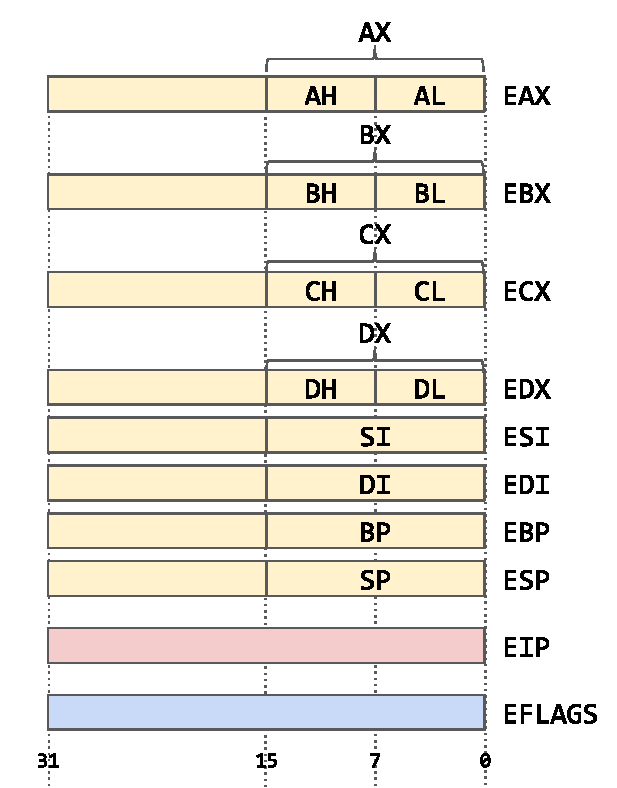
\includegraphics[width=\textwidth]{images/x86-isa}
			\end{figure}
		\end{column}
		\begin{column}{2.7in}
	      	\begin{itemize}
	      		\item General-purpose registers
	      		\begin{itemize}
	      			\item {\tt EAX}, {\tt EBX}, {\tt ECX}, {\tt EDX}
	      			\item {\tt ESI}, {\tt EDI} (source and destination index for string operations)
	      			\item {\tt EBP} (base pointer)
	      			\item {\tt ESP} (stack pointer)
	      		\end{itemize}
	      		\item Instruction pointer: {\tt EIP}
	      		\begin{itemize}
	      			\item No explicit access
	      			\item Modified by {\tt jmp}, {\tt call}, {\tt ret}
	      			\item Read through the stack (saved IP)
	      		\end{itemize}
	      		\item Program status and control: {\tt EFLAGS}
	      		\item (segment registers)
	      	\end{itemize}
    	\end{column}
  	\end{columns}
\end{frame}

\begin{frame}
	\frametitle{IA-32: {\tt EFLAGS} register}
  	\begin{itemize}
  		\item 32-bits register, boolean flags
  		\item \textbf{Program status}: overflow, sign, zero, auxiliary carry (BCD), parity, carry
  		\begin{itemize}
  			\item Indicate the result of arithmetic instructions
  			\item Extremely important for control flow
  		\end{itemize}
  		\item \textbf{Program control}: direction flag
  		\begin{itemize}
  			\item controls string instructions (auto-increment or auto-decrement)
  		\end{itemize}
  		\item \textbf{System}: control operating-system operations
  \end{itemize}
 \end{frame}

 \begin{frame}
	\frametitle{IA-32: {\tt EFLAGS} register}
	\begin{figure}
    	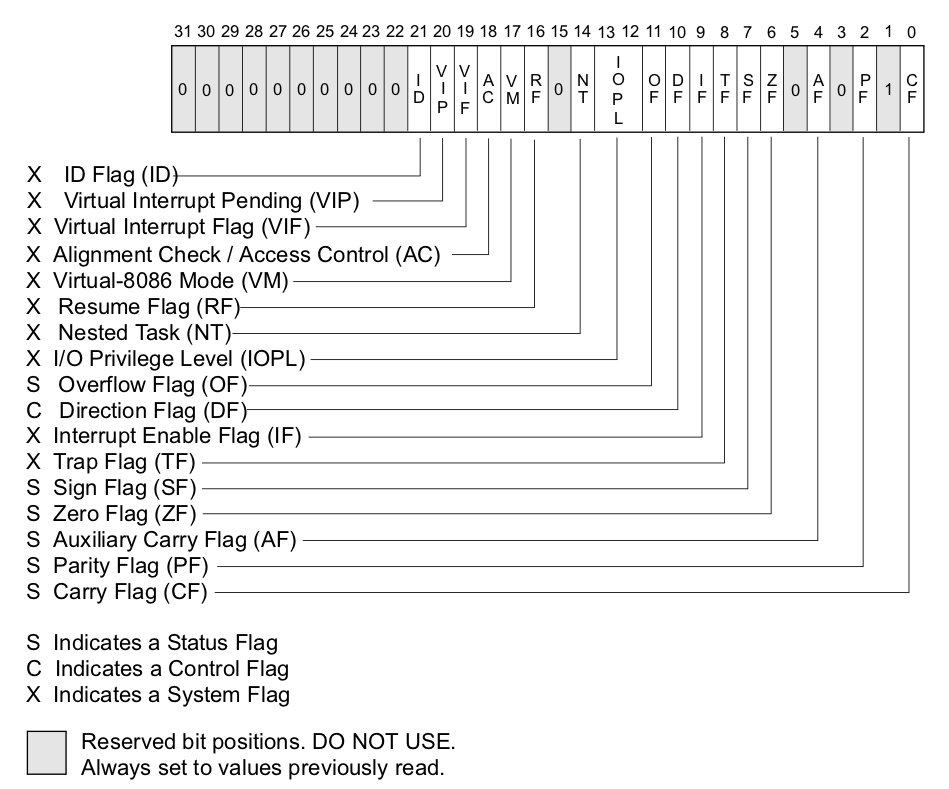
\includegraphics[height=2.8in]{images/intel-manual-eflags.png}
  	\end{figure}
\end{frame}

 \begin{frame}{Fundamental data types}

 \begin{description}
	\item[byte] 8 bits
	\item[word] 2 bytes
	\item[dword] Doubleword, 4 bytes (32 bits)
	\item[qword] Quadword, 8 bytes (64 bits)
 \end{description}

 \end{frame}
 
 \begin{frame}{Assembly and Machine Code}
 
 Assembly language: specific to each ISA, mapped to binary code
 
 	\begin{figure}
    	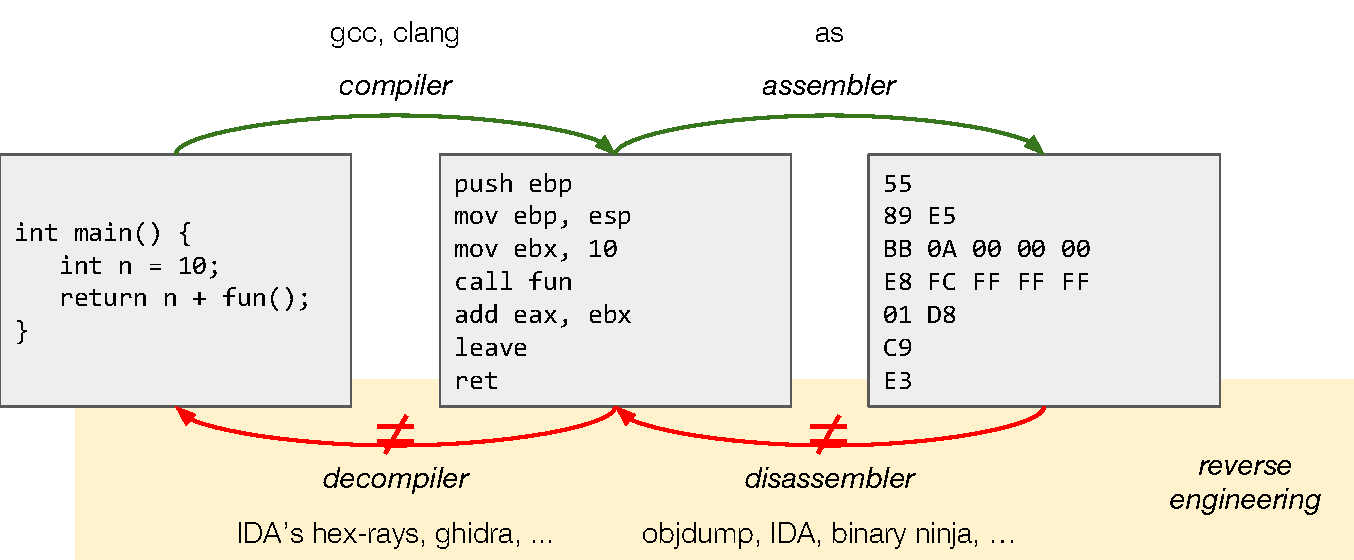
\includegraphics[width=\linewidth]{images/asm-disasm}
  	\end{figure}
For simplicity, we don't deal with the \emph{linking} process.
 \end{frame}

\begin{frame}{Assembly: Syntax}
	Two main syntaxes:
	\begin{itemize}
		\item \textbf{Intel}: default in most Windows programs (e.g.,~IDA)
		\item \textbf{AT\&T}: default in most UNIX tools (e.g.,~{\tt gdb}, {\tt objdump})
	\end{itemize}
	Beware: The order of the operands is \textbf{different} \\[.5em]
	We will use the Intel syntax
\end{frame}

\begin{frame}{Assembly: Syntax}
	\begin{center}
    	\emph{move the value 0 to \texttt{EAX}}
    	\par\vskip 0.8em\begin{tabular}{ccc}
      		\textbf{Intel} & $\qquad$ & \textbf{AT\&T} \\
      		\texttt{mov eax, 0h} & & \texttt{movl \$0x0,\%eax}\end{tabular}
  	\end{center}
	\vskip 1em
	\begin{center}
		\emph{move the value 0 to the address contained in \texttt{EBX}+4}
		\par\vskip 0.8em\begin{tabular}{ccc}
      		\textbf{Intel} & $\qquad$ & \textbf{AT\&T} \\
		\texttt{mov [ebx+4h],0h} & & \texttt{movl \$0x0,0x4(\%ebx)}\end{tabular}
	\end{center}
\end{frame}

\begin{frame}{x86: data movement}
\begin{block}{Examples}
\begin{tabular}{ll}
\multicolumn{2}{l}{Immediate to register:}\\
{\tt mov eax, 4h} & {\small EAX = 4} \\[.4em]
\multicolumn{2}{l}{Register to register:}\\
{\tt mov eax, ebx} & {\small EAX = EBX} \\[.4em]
\multicolumn{2}{l}{Memory to register (and register to memory):}\\
{\tt mov eax, [ebx]} & {\small EAX = *EBX} \\
{\tt mov eax, [ebx + 4h]} & {\small EAX = *(EBC + 4)} \\
{\tt mov eax, [edx + ebx*4 + 8]} & {\small EAX = *(EDX + EBX * 4 + 8)}
\end{tabular}
\end{block}
Note: memory to memory is an \textbf{invalid} combination\footnote{Except in some instructions, such as {\tt movs} (move from string to string).}
\end{frame}

\begin{frame}{x86 Assembly and Machine Code}
Instruction = opcode + operand

\begin{block}{Example}
	\centering
    	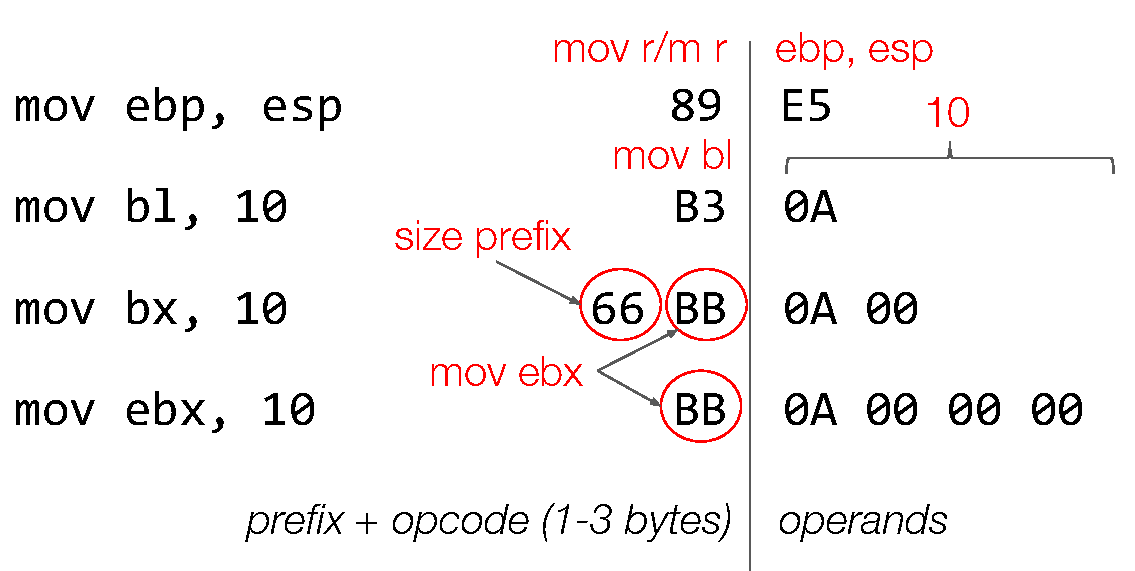
\includegraphics[width=.95\linewidth]{images/asm-machine-map}
\end{block}

Beware: in x86, instructions have \textbf{variable length}.
\end{frame}

\subsection{Basic Instructions}

%\begin{frame}
%  \frametitle{Instructions}
%  \begin{itemize}
%	  \item{Every processor has a large instruction set (see, e.g., Intel Software Developer's Manual\footnote{\url{https://software.intel.com/en-us/articles/intel-sdm}})}
%	  \item{A subset of the whole instruction set is usually processor dependent}
%	  \item{We will focus on a small subset of the general purpose x86 instructions}
%	  \item{We will use the Intel syntax}
%	  \item Very good reference: \url{http://ref.x86asm.net/geek32.html}
%  \end{itemize}
%\end{frame}

\begin{frame}{Basic instructions}
	\begin{itemize}
	  \item \textbf{Data Transfer}: {\tt mov}, {\tt push}, {\tt pop}, {\tt xchg}, {\tt lea}
	  \item \textbf{Integer Arithmetic}: {\tt add}, {\tt sub}, {\tt mul}, {\tt imul}, {\tt div}, {\tt idiv}, {\tt inc}, {\tt dec}
	  \item \textbf{Logical}: {\tt and}, {\tt or}, {\tt not}, {\tt xor}
	  \item \textbf{Control Transfer}: {\tt jmp}, {\tt jne}, {\tt call}, {\tt ret}
	  \item and lots more\dots
	\end{itemize}
\end{frame}

\begin{frame}{Data Transfer: {\tt mov}}
  \begin{itemize}
  \item {\tt mov} \underline{\textbf{destination}}, \underline{\textbf{source}}\\
        \textbf{source}: immediate, register, memory location\\
	\textbf{destination}: register or memory location\\
  \item Basic load/store operations
  \begin{itemize}
  	\item Register to register, register to memory, immediate to register, immediate to memory
  	\item Memory to memory is INVALID (in every instruction)
  \end{itemize}
  \end{itemize}

  \begin{block}{Examples}
  	\centering
      \begin{tabular}{c|c|c}
        {\tt MOV eax, ebx} & {\tt MOV eax, FFFFFFFFh} & {\tt MOV ax, bx}\\[.4em]
        {\tt MOV [eax],ecx} & {\tt MOV [eax],[ecx]} \color{red}NO!!! & {\tt MOV al, FFh}\\
      \end{tabular}
  \end{block}
  
\end{frame}

\begin{frame}{Integer Arithmetics: {\tt add} and {\tt sub}}
\begin{table}
	\centering
\begin{tabular}{l|l}
{\tt add} \underline{\textbf{destination}}, \underline{\textbf{source}} & {\tt sub} \underline{\textbf{destination}}, \underline{\textbf{source}} \\
dest $\leftarrow$ dest $+$ source & dest $\leftarrow$ dest $-$ source \\
\end{tabular}
\end{table}
  
  \begin{itemize}
  \item Addressing: \\
    \textbf{source}: immediate, register, memory location\\
    \textbf{destination}: register or memory location\\
    (the destination has to be at least as large as the source)
  \item Negate a value: {\tt neg} [op]
  \item Bitwise operations: {\tt and}, {\tt or}, {\tt xor}, {\tt not} work similarly
   \end{itemize}

  \begin{block}{Examples}
  	\centering
      \begin{tabular}{c|c|c}
        {\tt add esp, 44h} & {\tt add edx, cx} & {\tt add al, dh} \\[.4em]
        {\tt sub esp, 33h} & {\tt sub eax, ebx} & {\tt sub [eax], 1h} \\
      \end{tabular}
  \end{block}
\end{frame}

\begin{frame}{Integer Arithmetics: unsigned multiply ({\tt mul})}
  \begin{itemize}
  \item{{\tt mul} \underline{\textbf{source}}}\\
    \textbf{source}: register or memory location
  \item dest $\leftarrow$ implied\_op $\times$ source
  \item \textbf{Implied operands} according to the size of \textbf{source}
  	\begin{itemize}
  		\item First operand: {\tt AL}, {\tt AX}, or {\tt EAX}
  		\item Destination: {\tt AX}, {\tt DX:AX}, {\tt EDX:EAX} (double the size of \textbf{source})
  	\end{itemize}
  \item Signed multiply: {\tt imul}
  \end{itemize}

  \begin{block}{Example}
	  \begin{itemize}
	  	\item {\tt mul ebx}: {\tt EDX:EAX $\leftarrow$ EAX * EBX}
	  	\begin{itemize}
	  		\item most significant bits of the result in {\tt EDX}
	  		\item least significant bits of the result in {\tt EAX}
	  	\end{itemize}
	  	\item {\tt mul cx}: {\tt DX:AX $\leftarrow$ AX * CX}
	  	\item {\tt mul cl}: {\tt AX $\leftarrow$ AL * CL}
	  \end{itemize}
  \end{block}
\end{frame}

\begin{frame}{Integer Arithmetics: unsigned divide ({\tt div})}
  \begin{itemize}
  \item{{\tt div} \underline{\textbf{source}}}\\
    \textbf{source}: register or a memory location
  \item Computes quotient and remainder
  \item Implied operand: {\tt EDX:EAX} (according to the size of \textbf{source})
  \item Signed divide: {\tt idiv}
  \end{itemize}

  \begin{block}{Examples}
  \begin{itemize}
  \item {\tt div ebx} (4 bytes)
  	\begin{itemize}
  		\item {\tt EAX $\leftarrow$ EDX:EAX / EBX}
		\item {\tt EDX $\leftarrow$ EDX:EAX \% EBX}
  	\end{itemize}
  \item {\tt div bx} (2 bytes)
  	\begin{itemize}
  		\item {\tt AX $\leftarrow$ DX:AX / BX} $\qquad$ {\tt DX = DX:AX \% BX}
  	\end{itemize}
  \item {\tt div bl} (1 byte)
  	\begin{itemize}
  		\item {\tt AL $\leftarrow$ AX / BX} $\qquad$ {\tt AH = AX \% BX}
  	\end{itemize}
  \end{itemize}
  \end{block}
\end{frame}

\begin{frame}{Integer Arithmetics: {\tt cmp} and {\tt test}}
\begin{table}
	\centering
\begin{tabular}{l|l}
{\tt cmp} \underline{\textbf{op1}}, \underline{\textbf{op2}} & {\tt test} \underline{\textbf{op1}}, \underline{\textbf{op2}} \\
Computes op1 $-$ op2 & Computes op1 $\&$ op2 \\
\end{tabular}
\end{table}
  \begin{itemize}
	  \item Sets the flags ({\tt ZF},{\tt CF}, {\tt OF}, \dots)
	  \item Discards the result
  \end{itemize}

  \begin{block}{Examples}
  	\centering
      \begin{tabular}{c|c|c}
        {\tt cmp eax, ebx} & {\tt cmp eax, 44BBCCDDh} & {\tt cmp al, dh}\\[.4em]
        {\tt cmp al, 44h}&{\tt cmp ax,FFFFh} & {\tt cmp [eax],4h}\\
      \end{tabular}
  \end{block}
\end{frame}

\begin{frame}
  \frametitle{Control-Flow Instructions: conditional jumps}
  
  {\tt j<cc>} \underline{\textbf{address}} or \underline{\textbf{offset}}
  
  Jump to \textbf{address} if and only if a certain condition is verified
  
  \begin{columns}
    \begin{column}{2.5in}
      \begin{figure}
        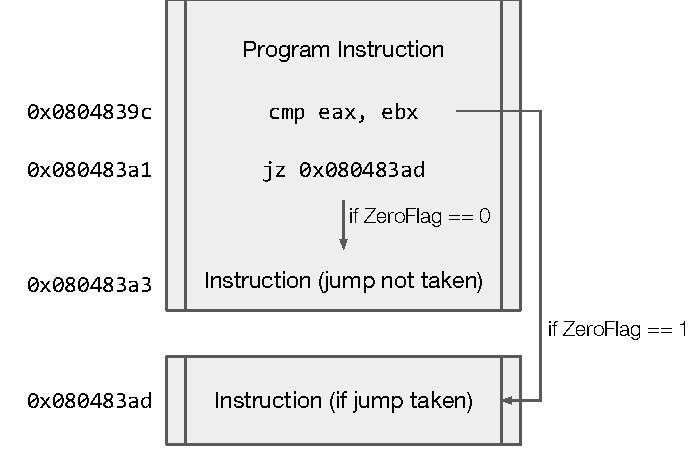
\includegraphics[width=\textwidth]{images/x86-jcc.pdf}
      \end{figure}
    \end{column}
    \begin{column}{2.5in}
	
     {\tt <cc>}: condition
      	\begin{itemize}
	   \item O,NO,S,NS,E,Z,NE, \dots
            \item based on one or more status flags of {\tt EFLAGS}
      \end{itemize}
      Examples:
      	\begin{itemize}
	\item {\tt jz} = jump if zero
	\item {\tt jg} = jump if greater than
	\item {\tt jlt} = jump if less than
	\end{itemize}
      Reference: \url{http://www.unixwiz.net/techtips/x86-jumps.html}
    \end{column}
  \end{columns}
\end{frame}

\begin{frame}
  \frametitle{Control-Flow Instructions: unconditional jump {\tt jmp}}
  \begin{columns}
    \begin{column}{0.4\columnwidth}
      \begin{figure}
        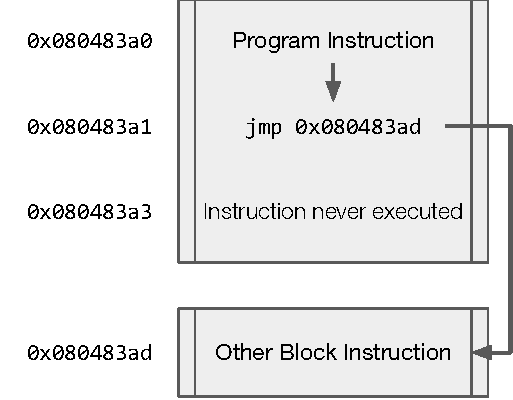
\includegraphics[width=1.1\textwidth]{images/x86-jmp.pdf}

        \label{Control Flow JMP}
      \end{figure}
    \end{column}
    \begin{column}{0.6\columnwidth}
      \begin{itemize}
	      \item{{\tt jmp} \underline{\textbf{address}} or \underline{\textbf{offset}}}\\
	      \item Unconditional jump: just set the {\tt EIP} to \textbf{address}
	      \item Can be also \emph{relative}: increment or decrement {\tt EIP} by an offset
      \end{itemize}
    \end{column}
  \end{columns}
\end{frame}

\begin{frame}[fragile]{Exercise 1}
  Translate the following C code in assembly x86. Assume EBX $\leftarrow$ \texttt{b}, ECX $\leftarrow$ \texttt{c}. Finally, \texttt{a} goes in EAX.
  \begin{lstlisting}[language={C}]
if (c == 0)
    a = b;
else
    a = -b;
  \end{lstlisting}
\end{frame}

\begin{frame}[fragile]{Solution}
  \begin{lstlisting}[language={[x86masm]Assembler}]
    mov     edx, 0
    cmp     ecx, edx
    jne     ELSE
    mov     eax, ebx
    jmp     ENDIF
ELSE:
    mov     eax, 0
    sub     eax, ebx
ENDIF:
    nop
    ...

\end{lstlisting}
\end{frame}

\begin{frame}[fragile]{Exercise 2}
  Translate the following C code in assembly x86. The variable \texttt{a} goes in EAX.
  \begin{lstlisting}[language={C}]
a = 0;
for(i = 0; i < 10; i++)
    a += i;
  \end{lstlisting}
\end{frame}

\begin{frame}[fragile]{Solution}
  \begin{lstlisting}[language={[x86masm]Assembler}]
    mov     eax, 0
    mov     ebx, 0
    mov     ecx, 10
LOOP:
    cmp     ebx, ecx
    jge     END
    add     eax, ebx
    inc     ebx
    jmp     LOOP
END:
    nop
    ...

\end{lstlisting}
\end{frame}

\begin{frame}[fragile]{A very simple example (what does it do?)}
Assume that the input is in registers: {\tt ECX} and {\tt EDX}; output: {\tt EAX}
\begin{lstlisting}[language={[x86masm]Assembler}]
    mov     eax, ecx
    mov     ebx, edx
    cmp     ebx, 0
    jz      LABEL
LOOP:
    cmp     ebx, 1
    jle     RET
    mul     ecx
    sub     ebx, 1
    jmp     LOOP
LABEL:
    mov     eax, 1
RET:
    ...
\end{lstlisting}
\end{frame}

\begin{frame}{Load effective address ({\tt lea})}
  \begin{itemize}
  		\item{{\tt lea} \underline{\textbf{destination}}, \underline{\textbf{source}}}\\
  		\textbf{source}: memory location\\
    	\textbf{destination}: register\\
  		\item{Like a {\tt mov}, but it is storing the pointer, not the value}
  		\item \alert{It does NOT access memory}
  \end{itemize}

  \begin{block}{Example}
  \par\noindent{}
  \centerline{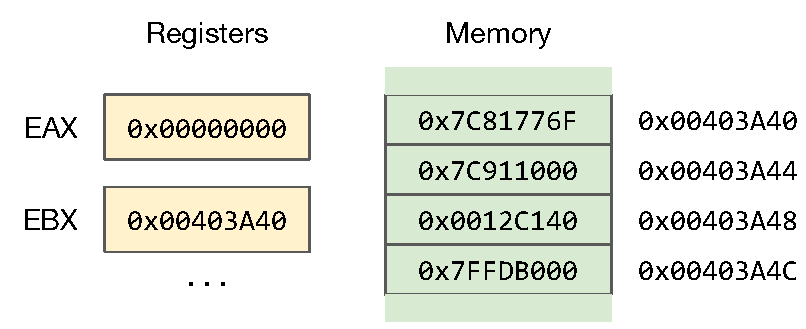
\includegraphics[width=0.7\textwidth]{images/x86-lea}}
  \centerline{\tt lea eax, [ebx + 8] $\rightarrow$ \texttt{EAX = 0x00403A48}}
  \centerline{\textbf{N.B.}: with {\tt mov eax, [ebx+8]} $\rightarrow$ {\tt EAX = 0x0012C140}}
   \end{block}
\end{frame}

\begin{frame}{Basic Instructions: {\tt nop}}
  \begin{itemize}
  \item{{\tt nop} = \textbf{No Operation}. Just move to next instruction.}
  \item{The opcode is pretty famous and is {\tt 0x90}}
  \item{Really useful in exploitation (we will see!)}
  \end{itemize}
\end{frame}

\begin{frame}{Interrupts and Syscalls}

  \begin{itemize}
  	\item {\tt int} \underline{\textbf{value}}
  		\begin{itemize} 
  			\item \textbf{value}: software interrupt number to generate (0-255)
  			\item Every OS has its set of interrupt numbers (e.g., {\tt 80h} for Linux system calls)
  		\end{itemize}
  	\item {\tt syscall} used for Linux 64-bit
  	\item {\tt sysenter} used by Microsoft Windows
  \end{itemize}
\end{frame}

\subsection{x86\_64}
\begin{frame}{The x86\_64 ISA}
  \centering
  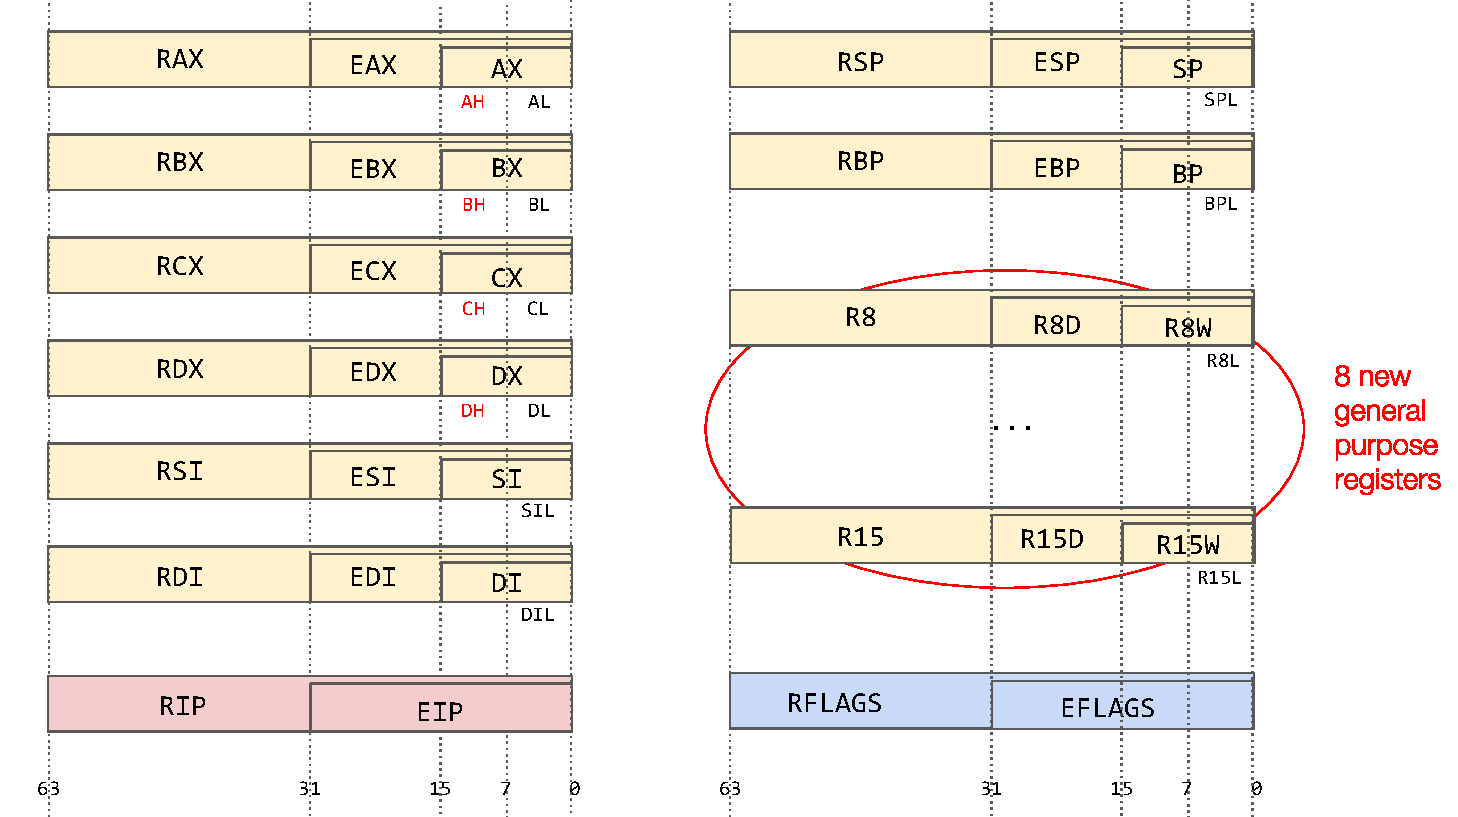
\includegraphics[width=1\linewidth]{images/x86-64}
\end{frame}

\begin{frame}
  \frametitle{Endianness}
  \textbf{Endianness}: convention that specifies in which order the bytes of a data word are lined up sequentially in memory.
  \begin{block}{Big-endian (left)}
  \begin{columns}
    \begin{column}{0.6\textwidth}
      Systems in which the \emph{most significant byte} of the word is stored in the \emph{smallest address} given.
    \end{column}
    \begin{column}{0.25\textwidth}
      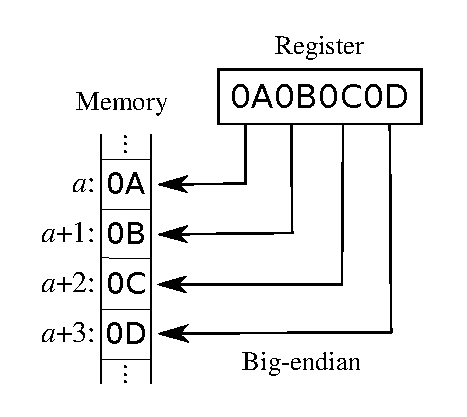
\includegraphics[width=\textwidth]{images/Big-Endian.pdf}
    \end{column}
  \end{columns}
  \end{block}
    \begin{block}{Little-endian}
  \begin{columns}
    \begin{column}{0.25\columnwidth}
      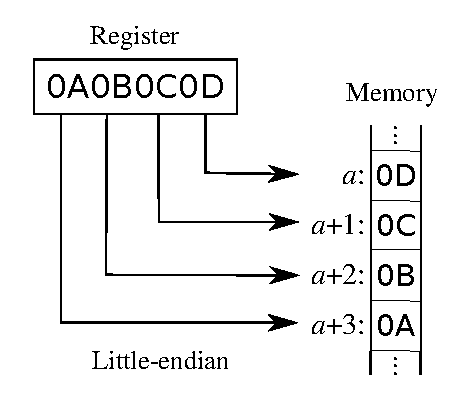
\includegraphics[width=\textwidth]{images/Little-Endian.pdf}
      \label{Little-Endian (right)}

    \end{column}
    \begin{column}{0.6\columnwidth}
      Systems in
      which the \emph{least significant} byte is stored in the
      \emph{smallest address}. \alert{IA-32 is ``little endian''}.

    \end{column}

  \end{columns}
  \end{block}
\end{frame}

%\begin{frame}
 % \frametitle{Endianness cont.}
%  The \textbf{endianness} is a convention that specifies in which order the bytes of a data word are lined up sequentially in memory.
%  \begin{columns}
%    \begin{column}{0.5\columnwidth}
%      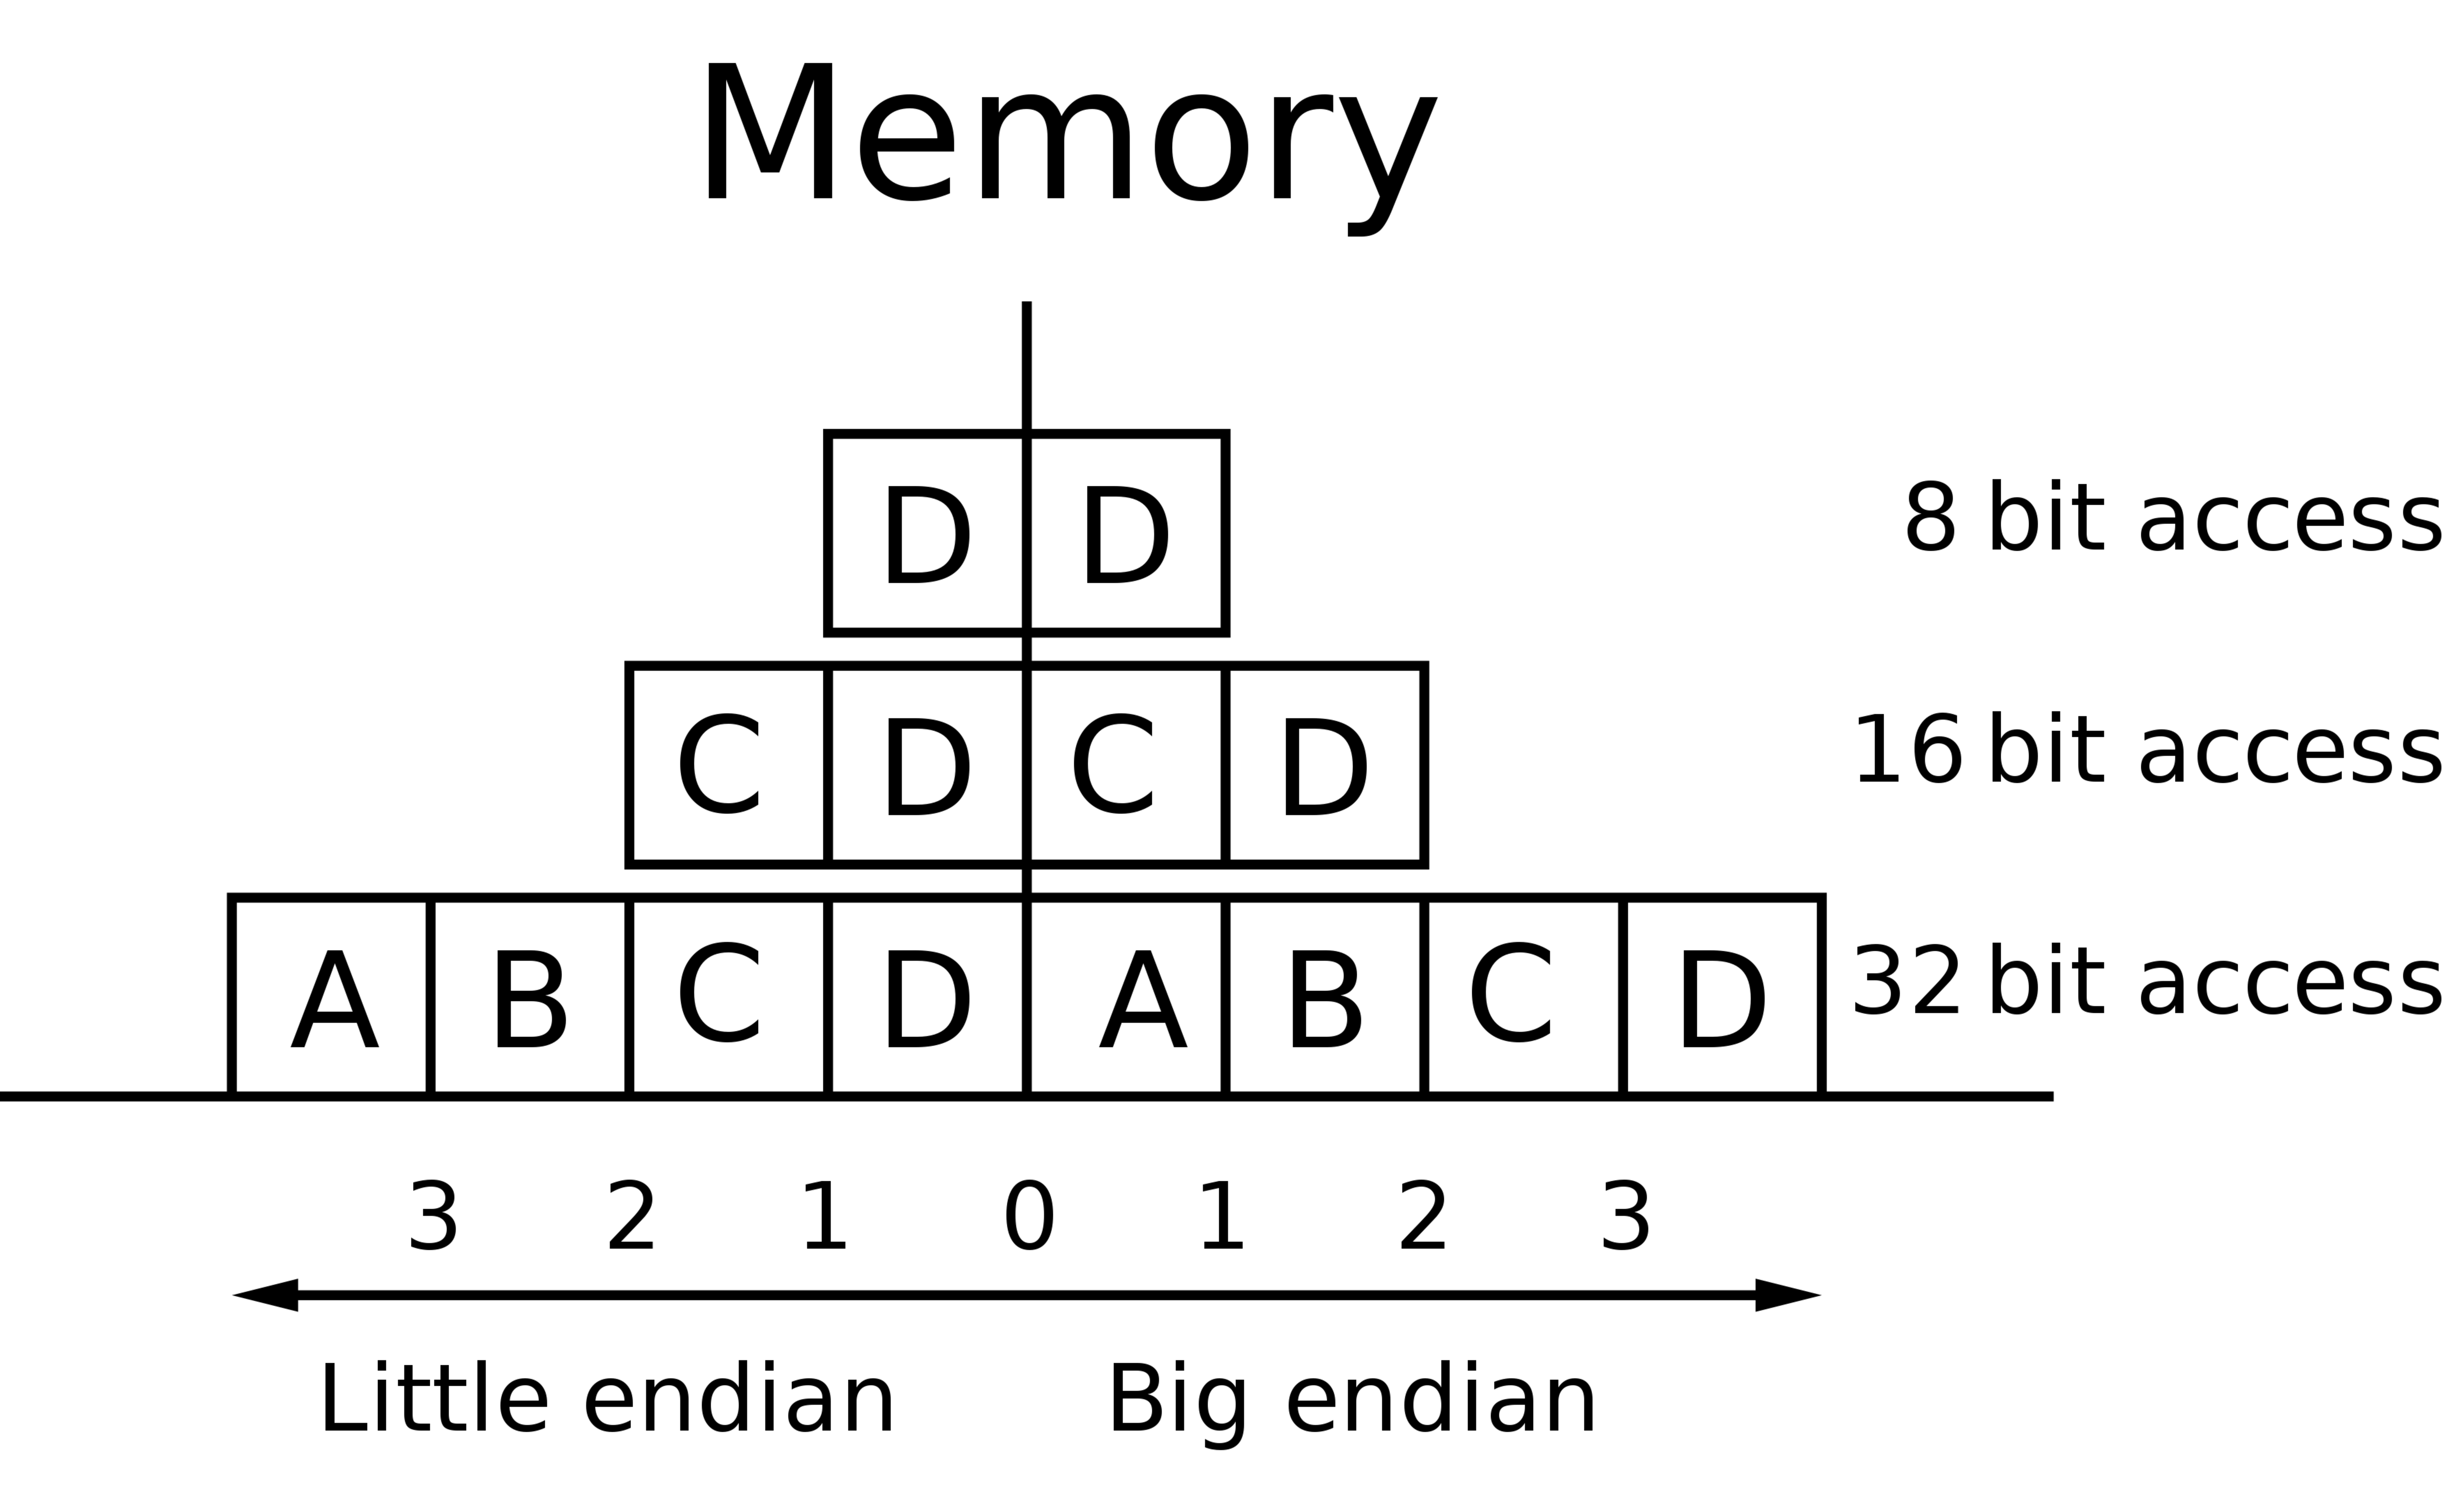
\includegraphics[width=\textwidth]{images/Endianessmap1.pdf}
%      \label{Big-Endian}
 %   \end{column}
 %   \begin{column}{0.5\columnwidth}
 %     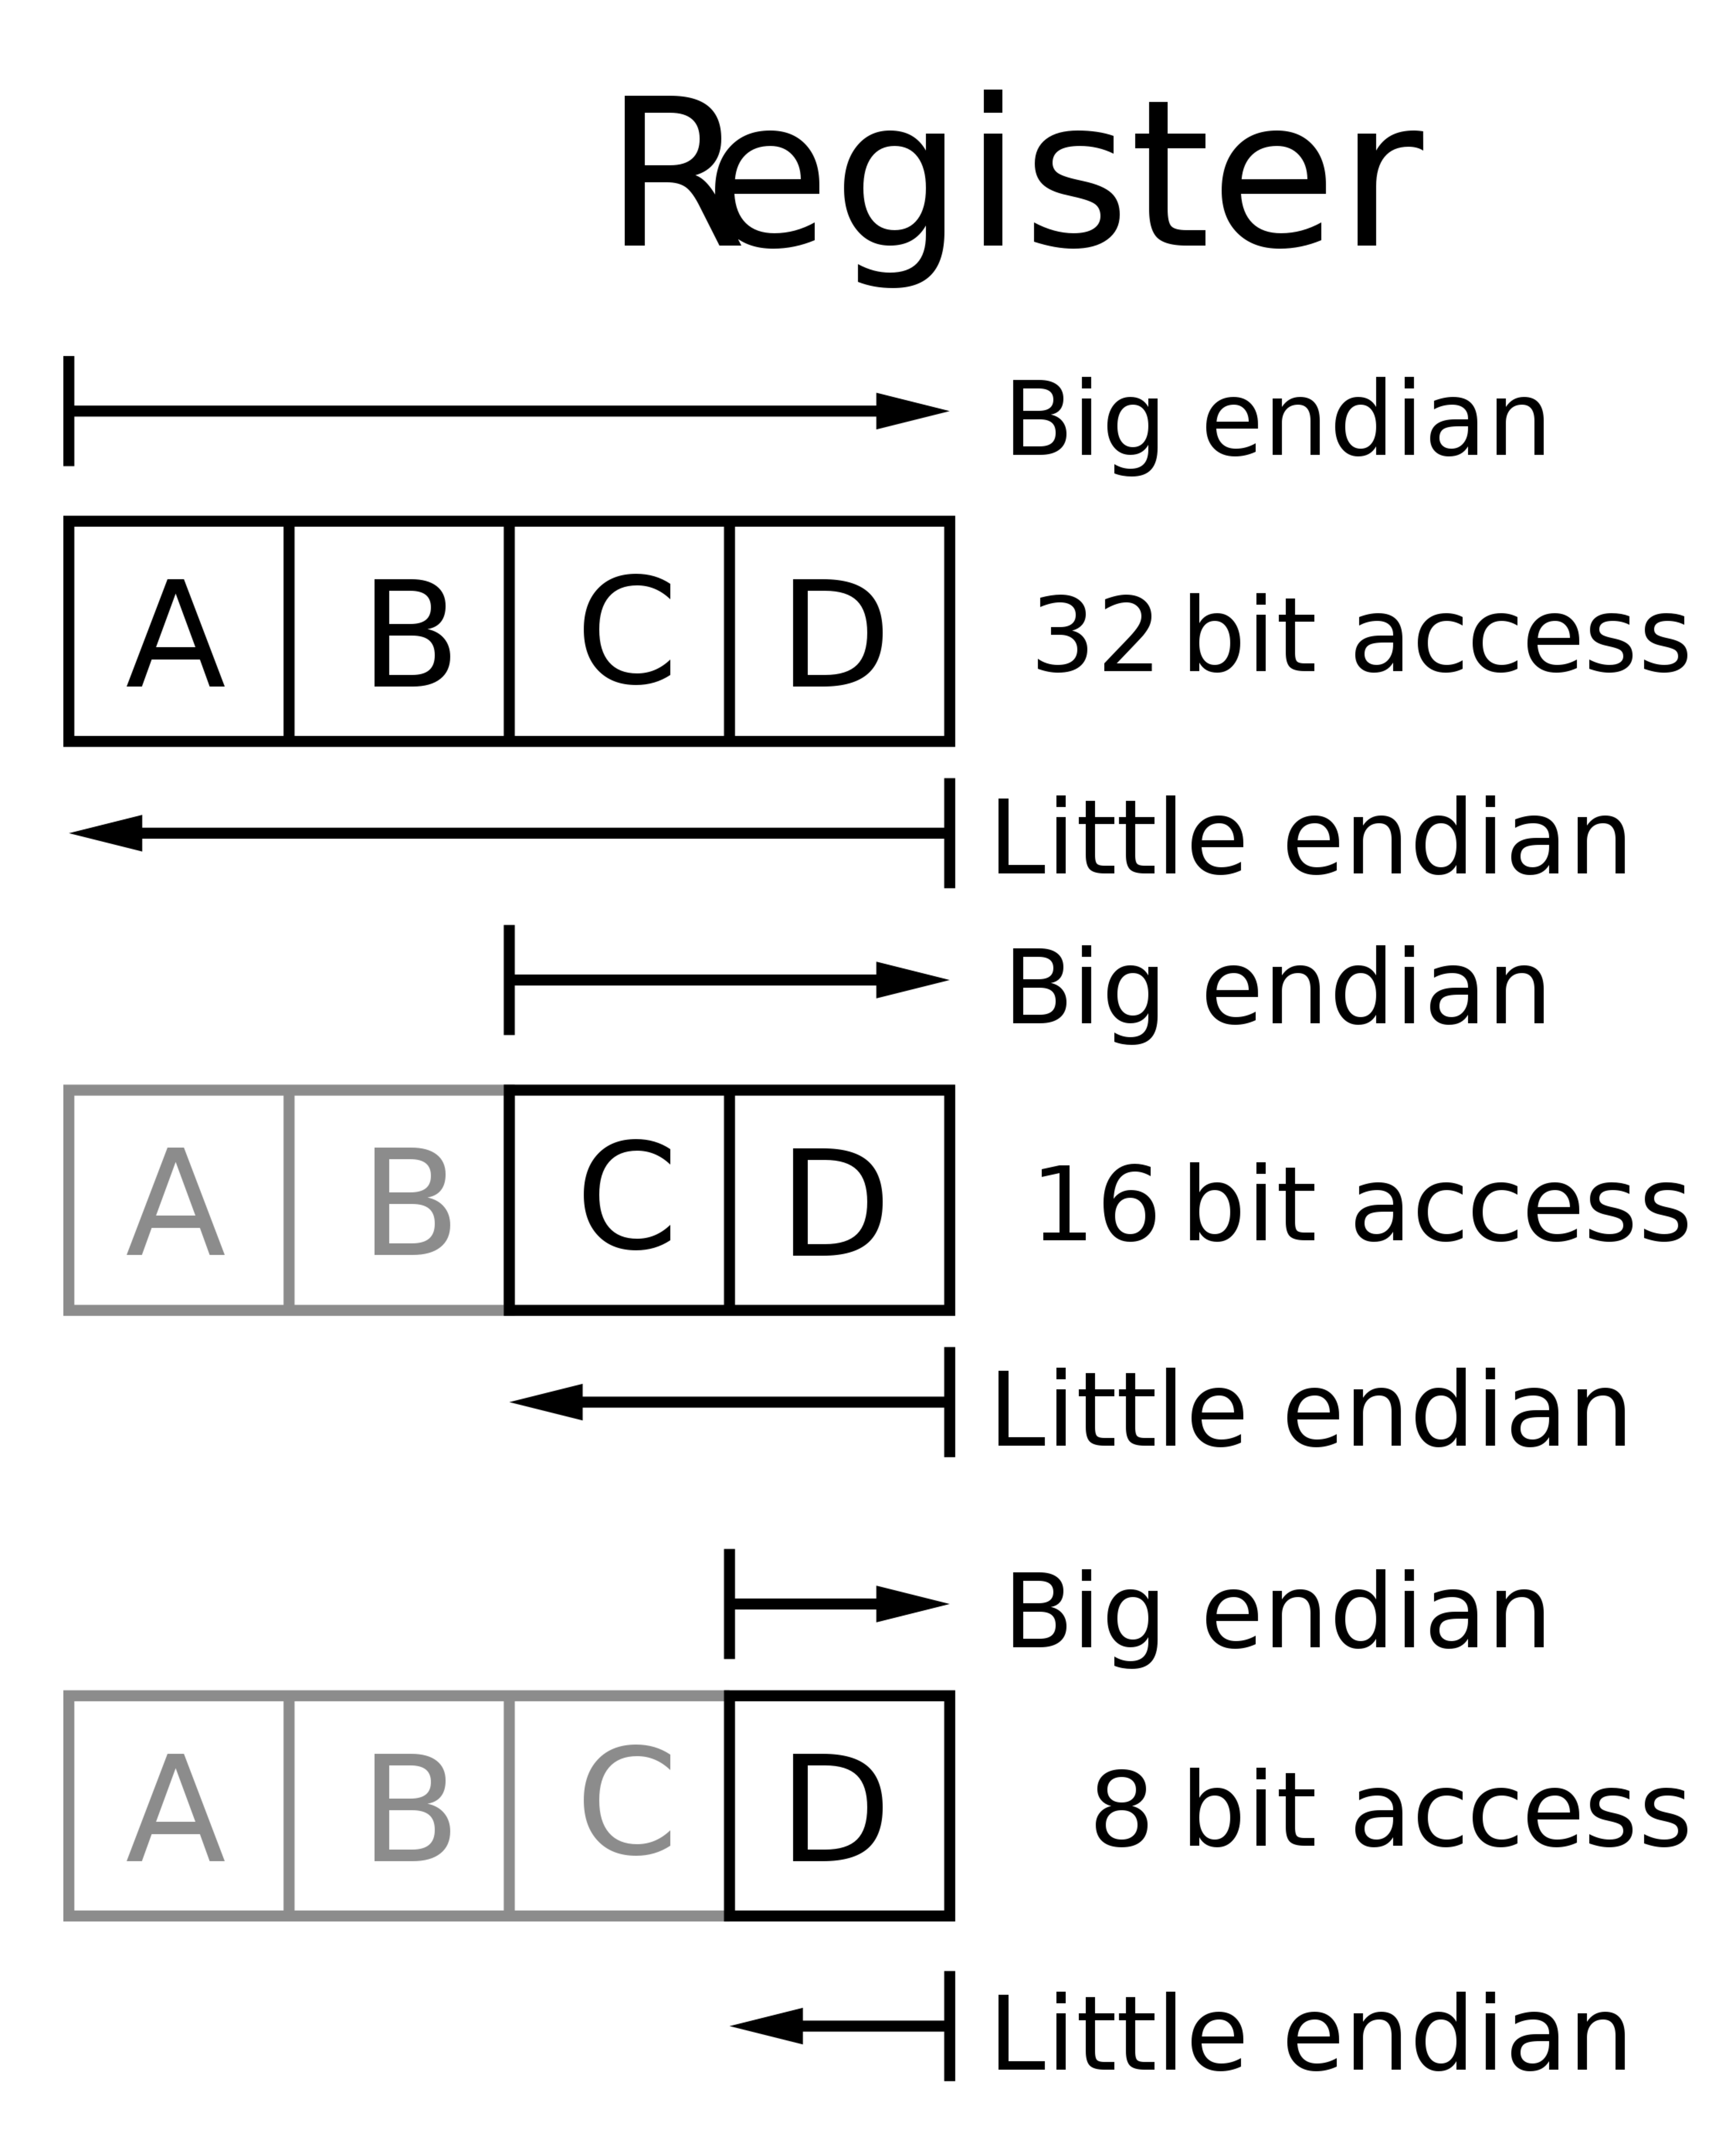
\includegraphics[width=0.6\textwidth]{images/Endianessmap2.pdf}
%      \label{Little-Endian}
%    \end{column}
%  \end{columns}
%\end{frame}

\section{Program Layout and Functions}

\subsection{Memory Layout}

\begin{frame}
  \frametitle{Binary File Formats}
  \begin{itemize}
  \item{\textbf{PE (Portable Executable):} used by Microsoft binary executables}
  \item{\textbf{ELF:} common binary format for Unix, Linux, FreeBSD and others}
  \item In both cases, we are interested in how each executable is
    mapped into memory, rather than how it is organized on disk.
  \end{itemize}
\end{frame}

\begin{frame}
  \begin{changemargin}{-1cm}{-1cm}
    \frametitle{How an executable is mapped to memory in Linux (ELF)}
    \begin{table}[l]
        \scalebox{0.7}{

          \begin{tabular}{ll}
            \toprule
            \textbf{Executable}&\textbf{Description}\\
            \midrule
            .plt& This section holds stubs which are responsible of \\
            &external functions linking.\\\midrule
            .text&This section holds the "text," or executable instructions, of a program.\\\midrule
            .rodata& This section holds read-only data that contribute to \\
            &the program's memory image\\\midrule
            .data& This section holds initialized data that contribute to \\
            &the program's memory image\\\midrule
            .bss&This section holds uninitialized data that contributes to the program's memory image.\\
            &By definition, the system initializes the data with zeros when the program begins to run.\\\midrule
            .debug&This section holds information symbolic debugging.\\\midrule
            .init&This section holds executable instructions that contribute to the process initialization code.\\
            &That is, when a program starts to run, the system arranges to execute the code in this\\
            &section before calling the main program entry point (called main for C programs).\\
            \midrule
            .got&This section holds the global offset table.\\
            \bottomrule

          \end{tabular}
      }
    \end{table}
  \end{changemargin}
\end{frame}

% \begin{frame}
%   \begin{changemargin}{-1cm}{-1cm}
%     \frametitle{How an executable is mapped to memory in Windows (PE)}
%     \begin{table}[l]
%         \scalebox{0.9}{
%           \begin{tabular}{ll}
%             \toprule
%             \textbf{Executable}&\textbf{Description}\\\midrule
%             .text&Contains the executable code\\\midrule
%             .rdata&Holds read-only data that is globally accessible within	\\
%             &the program\\\midrule

%             .data&Stores global data accessed throughout the program\\\midrule
%             .idata&stores the import function information;\\\midrule
%             .edata&stores the export function information;\\\midrule
%             .pdata&Present only in 64-bit executables and stores\\
%             & execption-handling information\\\midrule
%             .rsrc&Stores resources needed by the executable\\\midrule
%             .reloc&Contains information for relocation of library files\\\bottomrule
%           \end{tabular}
%       }
%     \end{table}
%   \end{changemargin}
% \end{frame}

\begin{frame}[fragile]{Simplified program memory layout}    
 \begin{center}
    {\footnotesize Low addresses ({\tt 0x80000000})}

    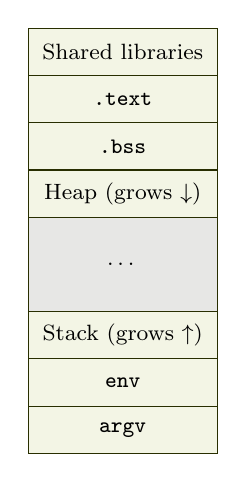
\begin{tikzpicture}[scale=0.6, font=\footnotesize]
    \cell{Shared libraries}
    \cell{{\tt .text}}
    \cell{{\tt .bss}}
    \cell{Heap (grows $\downarrow$)}
    \padding{2}{\dots}
    \cell{Stack (grows $\uparrow$)}
    \cell{{\tt env}}
    \cell{{\tt argv}}
    \end{tikzpicture}
    
    {\footnotesize High addresses ({\tt 0xbfffffff})}
    
\end{center}
\end{frame}
\subsection{The Stack}
\begin{frame}{The Stack}
\begin{itemize}
	\item LIFO (last in first out) data structure
	\item Used to manage functions
		\begin{itemize}
		\item local variables
		\item return addresses
		\item ...
		\end{itemize}
	\item Handled through the register {\tt ESP} (stack pointer)
	\item Remember: the stack grows \textbf{toward lower addresses} (downward the address space)
\end{itemize}
\end{frame}

\begin{frame}[fragile]{Stack Management Instructions: {\tt push}}
	\par\noindent{}
	\centerline{{\tt push} \underline{{\bf immediate}} or \underline{\bf register}}
	\par\noindent Stores the immediate or register value at the top of the stack and decrements the {\tt ESP} of the operand size
	
	\begin{block}{Example}
	\begin{columns}
	\begin{column}{0.45\textwidth}
	\only<-2>{Initial}\only<3->{Final} condition: {\tt EAX} = $30$ \\[.5em]
	{\tt push eax} \\[1em]
	is equivalent to: \\[1em]
	\alert<2>{{\small\tt sub esp, 4} \\}
	\alert<3>{{\small\tt mov DWORD PTR [esp], eax}}
	\end{column}
	
	\begin{column}{0.4\textwidth}
		\centering\par
		{\scriptsize Low addresses ({\tt 0x80000000})}\\[.5em]
		\begin{drawstack}[scale=0.7]
		\cell{}
		\only<2->{\bcell{\only<3->{$30$}}\cellptr{{\tt ESP}}}
		\only<-1>\cell{}
		\bcell{$100$} \only<1>{\cellptr{{\tt ESP}}}
		\end{drawstack}
		{\scriptsize High addresses ({\tt 0xbfffffff})}
	\end{column}	
	\end{columns}
	\end{block}
\end{frame}

\begin{frame}[fragile]{Stack Management Instructions: {\tt pop}}
	\par\noindent{}
	\centerline{{\tt pop} \underline{{\bf destination}}}
	\par\noindent Loads to the destination a word off the top of the stack, then it increases {\tt ESP} of the operand's size.

	\begin{block}{Example}
	\begin{columns}
	\begin{column}{0.45\textwidth}
	\only<-2>{Initial}\only<3->{Final} condition: {\tt EAX} = \only<-1>{???}\only<2->{$30$} \\[.5em]
	{\tt pop eax} \\[1em]
	is equivalent to: \\[1em]
	\alert<2>{{\tt mov eax, DWORD PTR [esp]} \\}
	\alert<3>{{\tt add esp, 4} \\}
	\end{column}
	
	\begin{column}{0.4\textwidth}
		\centering\par
		{\scriptsize Low addresses ({\tt 0x80000000})}\\[.5em]
		\begin{drawstack}[scale=0.7]
		\cell{}
		\only<-2>{\bcell{$30$}\cellptr{{\tt ESP}}}
		\only<3->{\cell{$30$}}
		\bcell{$100$}\only<3->{\cellptr{{\tt ESP}}}
		\end{drawstack}
		{\scriptsize High addresses ({\tt 0xbfffffff})}
	\end{column}	
	\end{columns}
	\end{block}
\end{frame}
\subsection{Functions}
\begin{frame}[fragile]{Calling a function}
	Instruction {\tt call}:
	\begin{itemize}
		\item Push to the stack the address of the next instruction
		\item Move the address of the first instruction of the callee into {\tt EIP}
	\end{itemize}
\begin{block}{Example: Let's call {\tt func}, located at 0x800bff00}
\vskip 0.4em
\begin{columns}
\begin{column}{0.45\textwidth}
	Equivalent to:
	\begin{itemize}
		\item \alert<2>{\tt push address(of the instruction after the call!)}
		\item \alert<3>{\tt jmp func}
	\end{itemize}
	(reminder: we can't read or set {\tt EIP} directly!)
\end{column}
\begin{column}{0.4\textwidth}
	{\scriptsize Low addresses ({\tt 0x80000000})}\\[.5em]
	\begin{drawstack}[scale=0.7, font=\footnotesize]
	\cell{}
	\cell{\only<2->{0x8001025}}\only<2->{\cellptr{\tt ESP}}
	\bcell{Stack top}\only<-1>{\cellptr{\tt ESP}}
	\end{drawstack}
	{\scriptsize High addresses ({\tt 0xbfffffff})}
	\only<-2>{EIP = 0x8001020}
	\only<3->{EIP = 0x800bff00}
\end{column}
\end{columns}
\end{block}
\end{frame}

\begin{frame}[fragile]{Returning from a function}
	Instruction {\tt ret}:
	\begin{itemize}
		\item Restores the return address saved by {\tt call} from the top of the stack
	\end{itemize}
\begin{block}{Example: let's return from {\tt func}}
\vskip 0.4em
\begin{columns}
\begin{column}{0.45\textwidth}
	Equivalent to:
	\begin{itemize}
		\item \alert<2>{\tt pop eip}
	\end{itemize}
	(reminde: we can't read or set {\tt EIP} directly!)
\end{column}
\begin{column}{0.4\textwidth}
	{\scriptsize Low addresses ({\tt 0x80000000})}\\[.5em]
	\begin{drawstack}[scale=0.7, font=\footnotesize]
	\cell{}
	\cell{\only<-1>{0x8001025}}\only<-1>{\cellptr{\tt ESP}}
	\bcell{Stack top}\only<2->{\cellptr{\tt ESP}}
	\end{drawstack}
	{\scriptsize High addresses ({\tt 0xbfffffff})}
	\only<2->{EIP = 0x8001025}
	\only<-1>{EIP = 0x800bff00}
\end{column}
\end{columns}
\end{block}
\end{frame}

\renewcommand{\finishframe}[1]{
  \draw[snake=brace, line width=0.6pt, segment amplitude=7pt]
  (-2,\value{cellnb}-0.5) -- (-2,\value{startframe}-0.5);
  \draw (-3cm,\value{cellnb}*0.5+\value{startframe}*0.5-0.5) node {#1};
}

\begin{frame}[fragile]{Functions and Stack Frames}
\begin{columns}
\begin{column}{0.45\linewidth}
\begin{itemize}
\item Stack frame = stack area allocated to a function
\item {\tt EBP} register: pointer to the beginning (base) of a function's frame
\item At the beginning of a function:
	\begin{itemize}
	\item Save EBP to stack
	\item Set {\tt EBP} to the address of the function's frame
	\end{itemize}
\end{itemize}
\end{column}
\begin{column}{0.4\linewidth}
	\par
	{\scriptsize Low addresses ({\tt 0x80000000})}\\[.5em]
	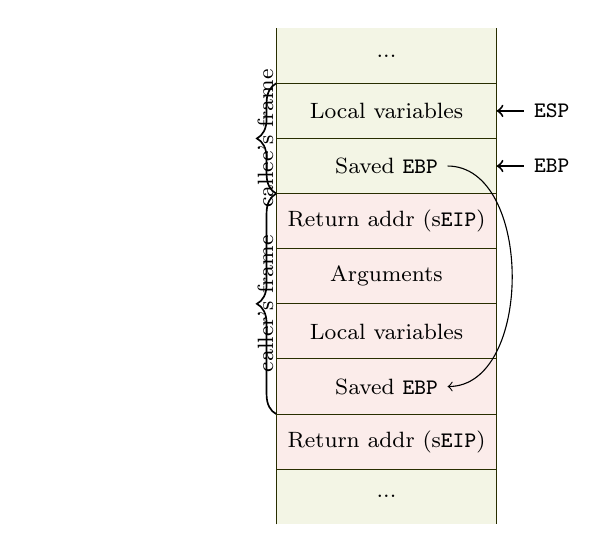
\begin{tikzpicture}[scale=.7, font=\footnotesize]
	\stacktop{}
	\startframe
	\cell{Local variables}\cellptr{{\tt ESP}} 
	\cell{Saved {\tt EBP}}\cellptr{{\tt EBP}} \coordinate (p1) at (currentcell.east);
	\finishframe{\rotatebox{90}{callee's frame}}
	\startframe
	\bcell{Return addr (s{\tt EIP})}
	\bcell{Arguments}
	\bcell{Local variables}
	\bcell{Saved {\tt EBP}} \coordinate (p2) at (currentcell.east);
	\finishframe{\rotatebox{90}{caller's frame}}
	\bcell{Return addr (s{\tt EIP})}
	\stackbottom
	\draw[->] (p1) to [bend left=90] (p2);
	\end{tikzpicture}
	{\scriptsize High addresses ({\tt 0xbfffffff})}
\end{column}
\end{columns}
\end{frame}

\begin{frame}[fragile]{Entering a function}
\begin{block}{Example: We've just called {\tt func}, located at 0x800bff00}
\vskip 0.4em
\begin{columns}
\begin{column}{0.35\textwidth}
	Setup the stack frame
	\begin{itemize}
		\item \alert<2>{\tt push ebp}
		\item \alert<3>{\tt mov ebp, esp}
	\end{itemize}
\end{column}
\begin{column}{0.4\textwidth}
	{\scriptsize Low addresses ({\tt 0x80000000})}\\[.5em]
	\begin{drawstack}[scale=0.7, font=\footnotesize]
	\startframe
	\cell{\only<2->{Saved EBP}}\only<2->{\cellptr{\tt ESP}}\only<3->{\cellptr{\tt EBP}}
	\cell{0x8001025}\only<1>{\cellptr{\tt ESP}}
	\finishframe{\rotatebox{90}{{\tt func}'s frame}}
	\bcell{\dots}
	\bcell{caller's sEBP}\only<-2>{\cellptr{\tt EBP}}
	\end{drawstack}
	{\scriptsize High addresses ({\tt 0xbfffffff})}
\end{column}
\end{columns}
\end{block}
\end{frame}

\begin{frame}[fragile]{Leaving a function}
Instruction {\tt leave}: restores the caller's base pointer
\begin{block}{Example: We're about to return from {\tt func}}
\vskip 0.4em
\begin{columns}
\begin{column}{0.35\textwidth}
	Equivalent to:
	\begin{itemize}
		\item \alert<2>{\tt mov esp, ebp}
		\item \alert<3>{\tt pop ebp}
	\end{itemize}
\end{column}
\begin{column}{0.4\textwidth}
	{\scriptsize Low addresses ({\tt 0x80000000})}\\[.5em]
	\begin{drawstack}[scale=0.7, font=\footnotesize]
	\startframe
	\cell{(... locals ...)}\only<1>{\cellptr{\tt ESP}}
	\cell{{Saved EBP}}\only<-2>{\cellptr{\tt EBP}}\only<2>{\cellptr{\tt ESP}}
	\cell{0x8001025}\only<3->{\cellptr{\tt ESP}}
	\finishframe{\rotatebox{90}{{\tt func}'s frame}}
	\bcell{\dots}
	\bcell{caller's sEBP}\only<3>{\cellptr{\tt EBP}}
	\end{drawstack}
	{\scriptsize High addresses ({\tt 0xbfffffff})}
\end{column}
\end{columns}
\end{block}
\end{frame}

\subsection{Calling Conventions}

\begin{frame}{Calling Conventions}
  \begin{itemize}
  	\item Defines
		\begin{itemize}
		\item how to pass parameters (stack, registers or both, and who is responsible to clean them up)
		\item how to return values
		\item caller-saved or callee-saved registers
		\end{itemize}
	\item The high-level language, the compiler, the OS, and the target architecture all together ``implement'' and ``agree upon'' a certain calling convention
    \begin{itemize}
    	\item it's part of the \alert{ABI}, the Application Binary Interface
    \end{itemize}
 \end{itemize}
\end{frame}


\begin{frame}{Calling Conventions: {\tt cdecl} (C declaration)}
  \begin{itemize}
  \item Default calling convention used by most x86 C compilers
  \begin{itemize}
  	\item Can be forced with the modifier \alert{\tt \_cdecl}
  \end{itemize}
  \item Arguments: passed \textbf{through the stack}, right to left order
  \item Cleanup: the \textbf{caller removes} the parameters from the stack \emph{after} the called function completes
  \item Return: register {\tt EAX}
  \item Caller-saved registers: {\tt EAX}, {\tt ECX}, {\tt EDX} (other are callee-saved)
  \end{itemize}
\end{frame}
\begin{frame}[fragile]
  \frametitle{{\tt cdecl}: Example}
\begin{lstlisting}[language=C]
void demo_cdecl(int a, int b, int c, int z);

//...

demo_cdecl(1, 2, 3, 4); //calling
\end{lstlisting}

\begin{lstlisting}[language={[x86masm]Assembler}]
; ...
push 4          ; push last parameter value
push 3          ; push third parameter value
push 2          ; ...
push 1
call demo_cdecl ; call the subroutine
add esp, 16  ; clean up the stack
\end{lstlisting}

\end{frame}

\begin{frame}[fragile]
  \frametitle{Calling Conventions: {\tt stdcall}}
  \begin{itemize}
  \item Microsoft's Win32 API standard calling convention (modifier: \alert{\tt \_stdcall}
  \item Parameters: passed using the stack (as in \_cdecl)
  \item Main difference: the callee is responsible for clearing the function parameters from the stack before returning
  \begin{itemize}
  \item To do this, the function needs to know the right number of parameter passed $\rightarrow$ can be used only with functions having a fixed number of parameters (e.g., no \texttt{printf}).
  \end{itemize}
  \end{itemize}

\begin{lstlisting}[language=C]
void _stdcall demo_stdcall(int a, int b, int c);
demo_stdcall(1, 2, 3);
\end{lstlisting}
\begin{lstlisting}[language={[x86masm]Assembler}]
ret 12  ; return and clear 12 bytes from the stack
\end{lstlisting}
\end{frame}

\begin{frame}[fragile]
  \frametitle{{\tt stdcall}: Example}
  \begin{columns}
    \begin{column}{.5\textwidth}
\begin{lstlisting}[language=C]
void function (int a, int b) {
  int array [5];
}

int main (int argc, char** argv) {
  function(1, 2);
  printf("This is where the ret address points");
}
\end{lstlisting}
    \end{column}
    \begin{column}{.5\textwidth}
    	\centering
    	\par{\scriptsize Low addresses ({\tt 0x80000000})}\\[.5em]
	\begin{drawstack}[scale=0.7, font=\footnotesize]
	\startframe
	\cell{array[0]}
	\padding{1}{...}
	\cell{array[4]}
	\cell{Saved EBP}
	\cell{Return address}
	\cell{1}
	\cell{2}
	\end{drawstack}
	\par{\scriptsize High addresses ({\tt 0xbfffffff})}
     \end{column}
  \end{columns}
\end{frame}

\begin{frame}[fragile]
  \frametitle{Assembler-level View of the Same Example}
  \begin{columns}
    \begin{column}{.5\textwidth}

\begin{lstlisting}[language={[x86masm]Assembler},basicstyle=\tiny\ttfamily]
public main
main proc near
push ebp
mov ebp, esp ; create stack
and esp,0FFFFFFFF0h
sub esp,10h ; make room for vars
mov dword ptr[esp+4],2 ; push 2
mov dword ptr[esp],1 ; push 1
call function
mov dword ptr [esp], offset format; "This is..."
call _printf
leave
ret
main endp

public function
function proc near
push ebp
mov ebp,esp ; create stack
sub esp,14h ; make room for array
leave
retn 8 ; remove 2 dwords
function endp
\end{lstlisting}
    \end{column}

    \begin{column}{.5\textwidth}
    	\centering
    	\par{\scriptsize Low addresses ({\tt 0x80000000})}\\[.5em]
	\begin{drawstack}[scale=0.7, font=\footnotesize]
	\startframe
	\cell{array[0]}
	\padding{1}{...}
	\cell{array[4]}
	\cell{Saved EBP}
	\cell{Return address}
	\cell{1}
	\cell{2}
	\end{drawstack}
	\par{\scriptsize High addresses ({\tt 0xbfffffff})}
     \end{column}
  \end{columns}
  \begin{figure}
  \end{figure}
\end{frame}

\begin{frame}[fragile]
  \frametitle{Calling Conventions: {\tt fastcall}}
  \begin{itemize}
  \item Modifier: \alert{\_fastcall}
  \item Up to 2 parameters passed via registers: {\tt ECX} and {\tt EDX}
  \item Other parameters pushed to the stack (right to left order, stack cleanup by callee as in {\tt stdcall})
  \end{itemize}
\begin{lstlisting}[language={[x86masm]Assembler}]
; demo_fastcall(1, 2, 3, 4);
push 4 ; push 4th parameter
push 3 ; push 3rd parameter
mov edx, 2 ; move 2nd parameter in EDX
mov ecx, 1 ; move 1st parameter in ECX
call demo_fastcall
; do not clean up the stack (done by callee)
\end{lstlisting}
\end{frame}

\begin{frame}{Calling Conventions: Linux x86-64 (System V ABI)}
\begin{itemize}
\item Parameters passed {\bf in registers}: {\tt rdi}, {\tt rsi}, {\tt rdx}, {\tt rcx}, {\tt r8}, {\tt r9}, subsequent ones on the stack (reverse order, caller cleanup)
\item Callee-saved registers: {\tt rbx}, {\tt rsp}, {\tt rbp}, {\tt r12}, {\tt r13}, {\tt r14}, and {\tt r15}
\item Caller-saved registers (scratch): {\tt rax}, {\tt rdi}, {\tt rsi}, {\tt rdx}, {\tt rcx}, {\tt r8}, {\tt r9}, {\tt r10}, {\tt r11}
\item Return value: {\tt rax} (if 128-bit: {\tt rax} and {\tt rdx})
\end{itemize}
\end{frame}

\begin{frame}[fragile]
  \frametitle{Linux x86-64 calling convention: Example}
  \begin{columns}
    \begin{column}{.5\textwidth}
\begin{lstlisting}[language={[x86masm]Assembler},basicstyle=\tiny\ttfamily]
main:
  push    rbp
  mov     rbp, rsp
  sub     rsp, 16
  mov     DWORD PTR [rbp-4], edi
  mov     QWORD PTR [rbp-16], rsi
  mov     esi, 2    ; Second parameter
  mov     edi, 1    ; First parameter
  call    function
  mov     esi, eax  ; Return value -> first param
  mov     edi, OFFSET FLAT:.LC0 ; "The return ...
  mov     eax, 0
  call    printf
  leave
  ret

function:
  push    rbp
  mov     rbp, rsp
  mov     DWORD PTR [rbp-4], edi
  mov     DWORD PTR [rbp-8], esi
  mov     edx, DWORD PTR [rbp-4]
  mov     eax, DWORD PTR [rbp-8]
  add     eax, edx
  pop     rbp
  ret
\end{lstlisting}
    \end{column}

    \begin{column}{.5\textwidth}

\begin{lstlisting}[language=C,basicstyle=\tiny\ttfamily]
int function (int a, int b) {
    return a + b;
}

int main (int argc, char** argv) {
    return printf("The return value is %d\n", function(1,2));
}
\end{lstlisting}
	\vspace{-2em}
	\begin{center}
    	\par{\scriptsize Low addresses}\\[.5em]
	\resizebox{!}{9em}{%
	\begin{drawstack}[scale=0.7, font=\footnotesize]
	\cell{2}
	\cell{1}
	\cell{Saved RBP}
	\cell{Return address}
	\end{drawstack}}
	\par{\scriptsize High addresses}
	\end{center}
    \end{column}
  \end{columns}
\end{frame}

\section{Tooling}
\begin{frame}
  \frametitle{Shell for Dummies \footnote{\texttt{cmd -{}-help} or \texttt{cmd -h} to get the aviable options}}
  \hspace*{-11mm}
  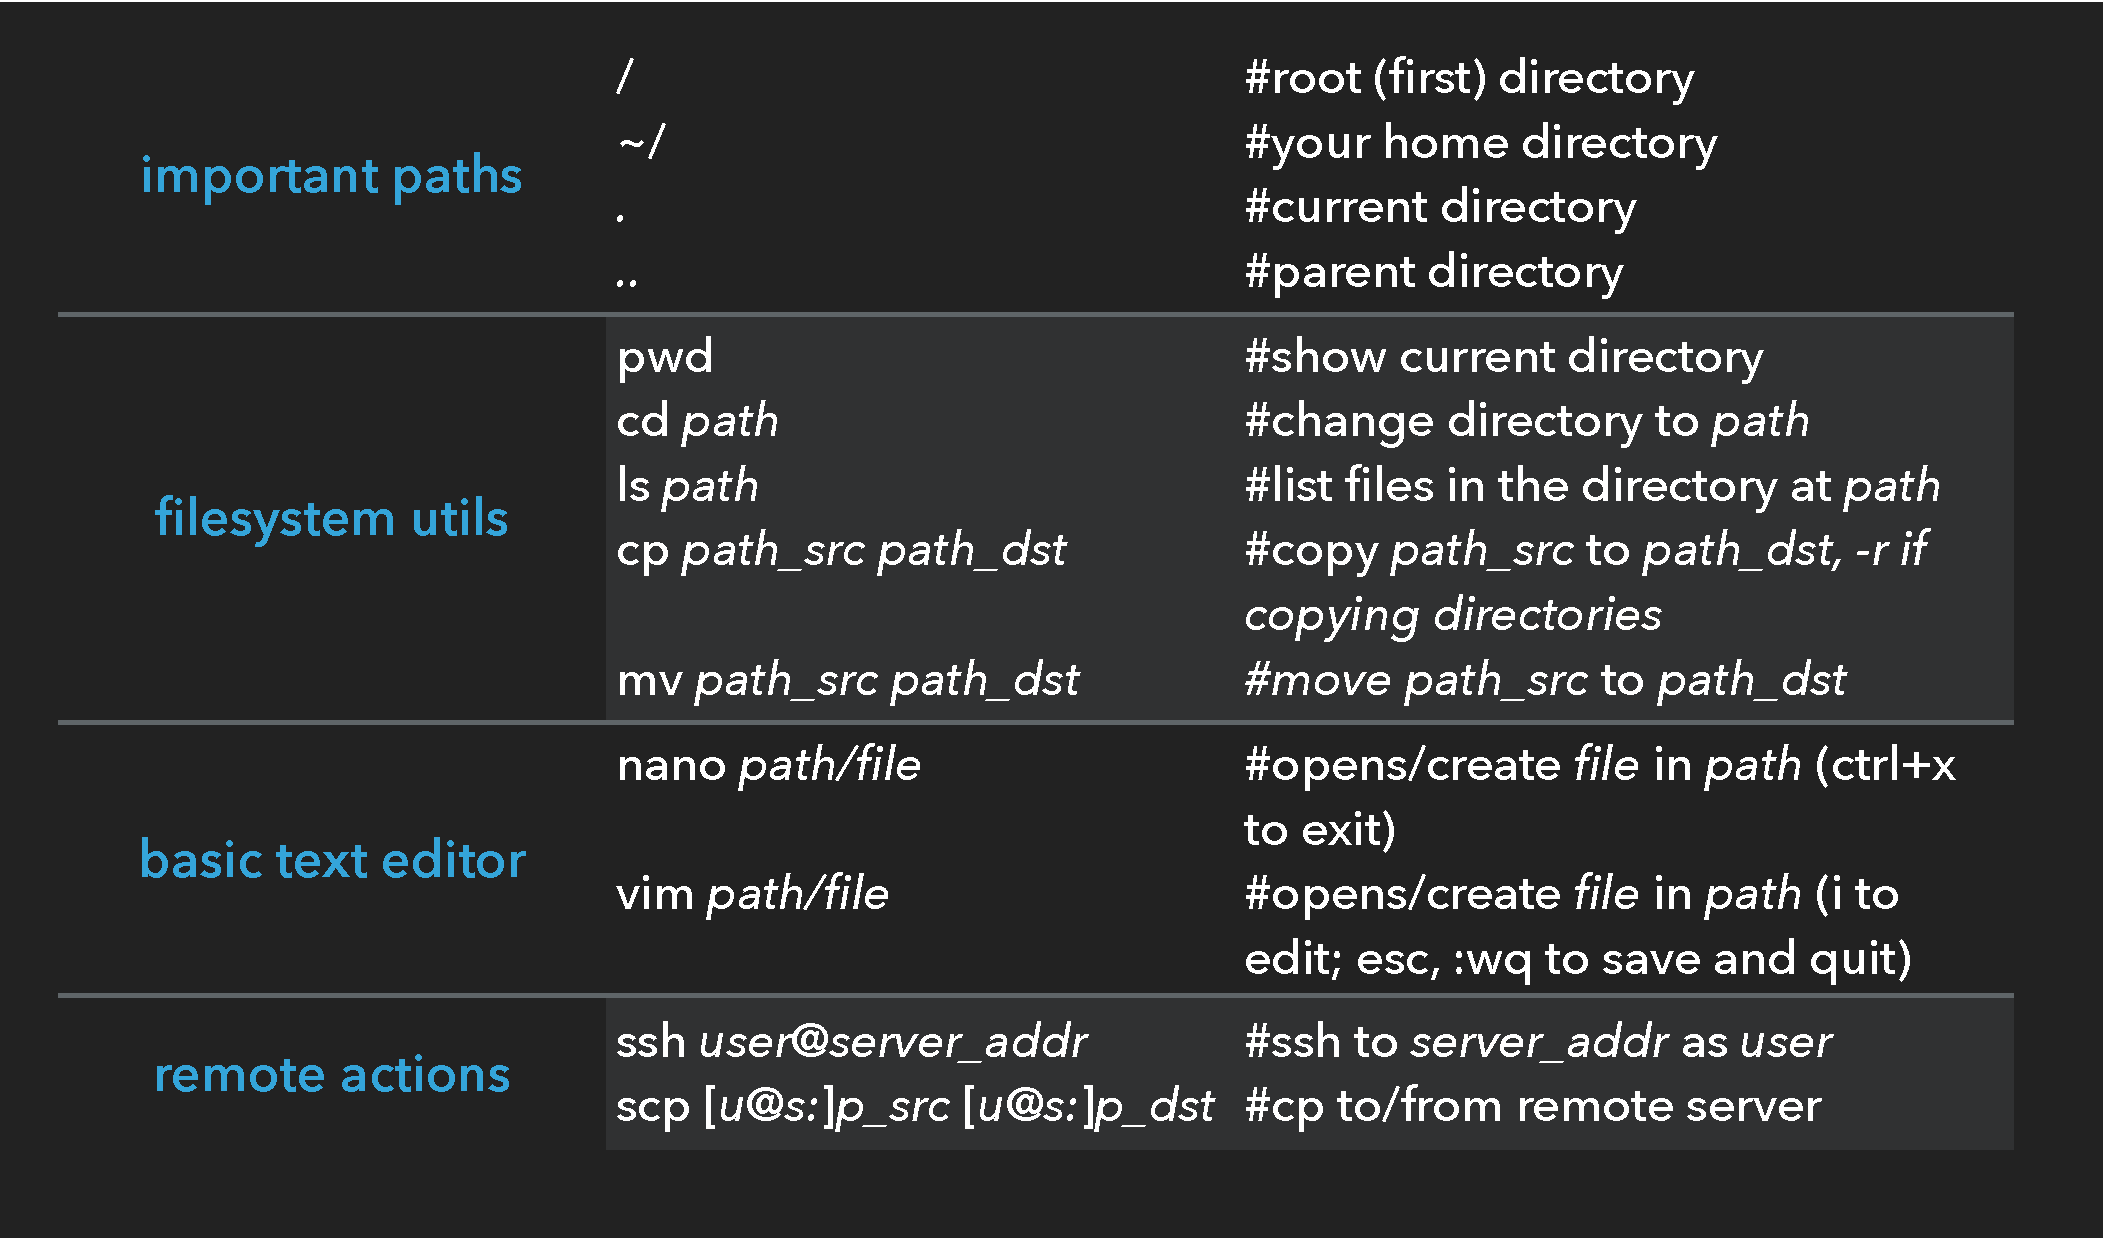
\includegraphics[width=\paperwidth]{./images/shell_1.pdf}
\end{frame}

\begin{frame}
  \frametitle{Shell for Dummies \footnote{\texttt{cmd -{}-help} or \texttt{cmd -h} to get the aviable options}}
  \hspace*{-11mm}
  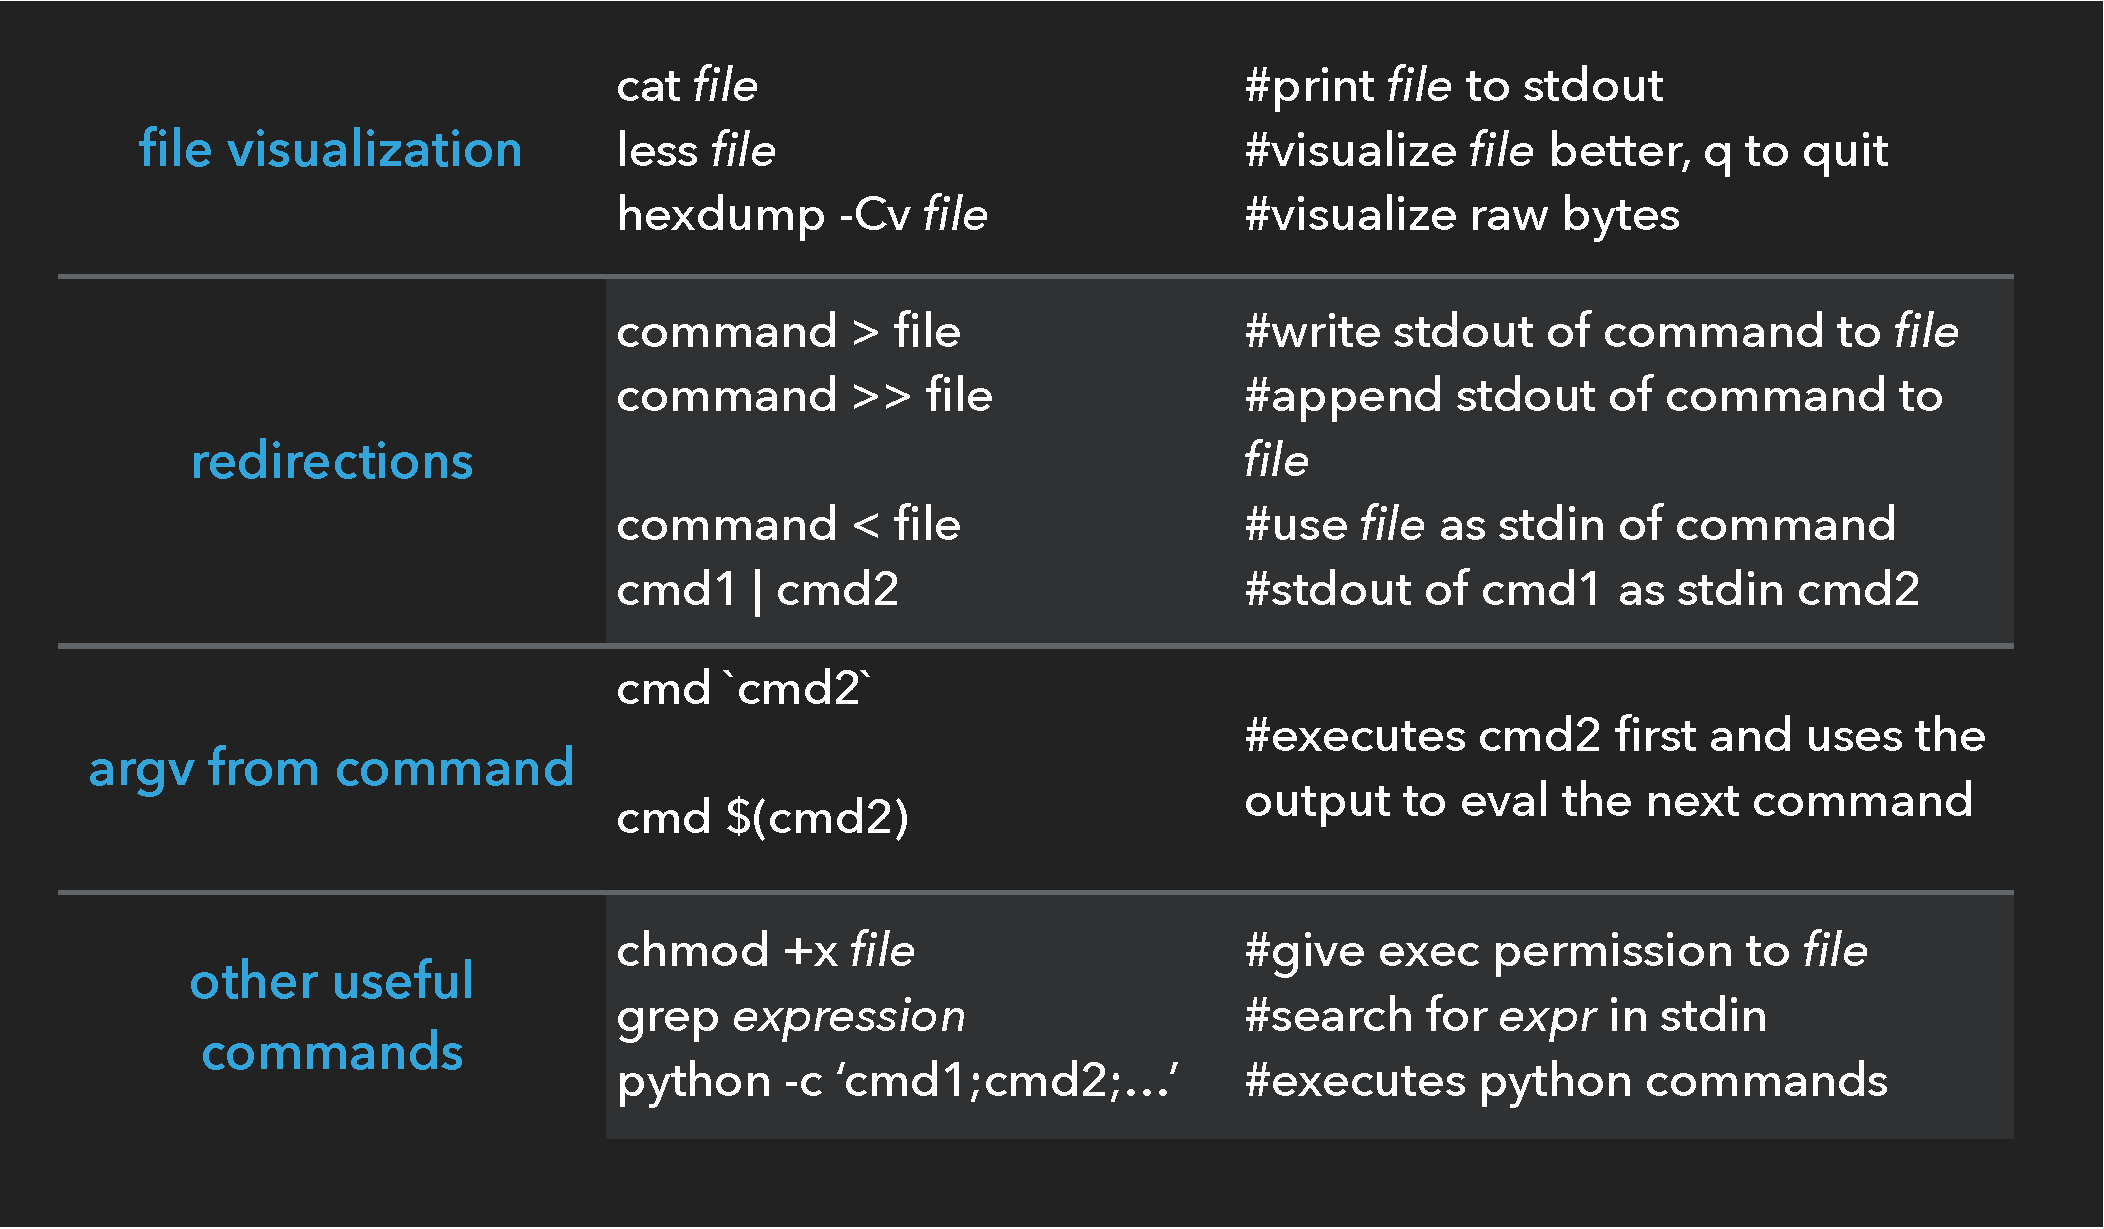
\includegraphics[width=\paperwidth]{./images/shell_2.pdf}
\end{frame}

\begin{frame}
  \frametitle{objdump}
  \begin{itemize}
  \item{{\tt man objdump}}\\
objdump \textbf{displays information} about one or more \textbf{object files}.
  \item{\texttt{-x}} all-headers
  \item{\texttt{-d}} disassemble
  \item{\texttt{-M intel}} intel syntax (default is AT\&T)
  \end{itemize}
\end{frame}

\begin{frame}
  \frametitle{Debugging: GDB}
  \begin{itemize}
  \item{{\bf What is GDB?}}\\
    GDB is GNU Project's Debugger: allows to follow, step by step, at assembler-level granularity, a running program, or what a program was doing right before it crashed.\footnote{http://www.gnu.org/software/gdb/}
  \end{itemize}
\end{frame}


% \begin{frame}
%   \frametitle{Shell For Dummies}
%   \resizebox{\linewidth}{!}{
%   \begin{tabular}{ l l p{6cm}}
%       \multirow{3}{3cm}{\textbf{file visualization}} & \texttt{cat file} & \#print file to stdout \\ 
%                                                    & \texttt{less file} & \#visualize file better, q to quit \\ 
%                                                    & \texttt{hexdump -Cv file} & \#visualize raw bytes \\ 
%       \hline
%       \multirow{4}{3cm}{\textbf{redirections}} & \texttt{command > file} & \#write stdout of command to file \\ 
%                                              & \texttt{command >> file} & \#append stdout of command to file \\ 
%                                              & \texttt{command < file} & \#use file as stdin of command \\ 
%                                              & \texttt{cmd1 | mcd2} & \#stdout of cmd1 as stdin cmd2 \\ 
%       \hline
%       \multirow{2}{3cm}{\textbf{argv from command}} & \texttt{cmd \textasciigrave cmd2\textasciigrave } & \#executes cmd2 first and uses the \\ 
%        & \texttt{cmd \$(cmd2)}    & output to eval the next command\\ 
%       \hline
%       \multirow{3}{3cm}{\textbf{other usefull commands}} & \texttt{command > file} & \#write stdout of command to file \\ 
%                                              & \texttt{command >> file} & \#append stdout of command to file \\ 
%                                              & \texttt{command < file} & \#use file as stdin of command \\ 

%     \end{tabular}
%   }
% \end{frame}

\begin{frame}
  \frametitle{Start, break and navigate the execution with gdb}
  \begin{itemize}
  \item{Suppose you have an executable binary and want run it}\\
    \begin{itemize}
    \item{{\bf gdb /path/to/executable} loads the binary in gdb}
    \end{itemize}
  \item{Now you decide to start the program with two parameters}\\
    \begin{itemize}
    \item{{\bf run 1 "abc"} passes 1 via \path|argv[1]| and
        \path|"abc"| as \path|argv[2]|}
    \item \textbf{run `printf "AAAAAAAAAAAA"`} (with the back ticks)
      we're passing the output of the print (very useful when you need
      to pass non printable characters such as raw bytes)
    \end{itemize}
  \item{Suppose you want to stop the execution at the address of a
      certain instruction}
    \begin{itemize}
    \item{{\bf break *0xDEADBEAF} places a break point at that address}
    \item{{\bf break *main+1} with debugging symbols this can be less painful}
    \item{{\bf catch syscall} block the execution when a syscall happens}
    \end{itemize}
  \end{itemize}
\end{frame}

\begin{frame}
  \frametitle{Start, break and navigate the execution with gdb}
  \begin{itemize}
  \item{Now the execution stops at our break point. Here we
      can do several things}
  \item{Examples:}
    \begin{itemize}
    \item{{\bf ni} allows to procede instruction per instruction}
    \item{{\bf next 4} moves 4 lines ahead (if you have the
        line-numbers information in the binary)}
    \item{{\bf si} step into function}
    \item{{\bf finish} run until the end of current function}
    \item{{\bf continue} runs until the next break point (if any)}

    \end{itemize}
  \item{To see info about the execution state:}
    \begin{itemize}
    \item{{\bf info registers} to inspect the content of the registers}
    \item{{\bf info frame} to see the values of the stack frame
        related to the function where we are in}
    \item{{\bf info file} print the information about the sections of the binary}
    \end{itemize}
  \end{itemize}
\end{frame}

\begin{frame}
  \frametitle{Navigate the stack}
  \begin{itemize}
  \item{Suppose we're stopped somewhere in the code and want to
      inspect the stack}
  \item{Some useful view of the stack is achievable with:}
    \begin{itemize}
    \item{{\bf x/100wx \$esp} prints 100 words of memory from the address found in the ESP to ESP+100 (x = hexadecimal formatting)}
    \item{{\bf x/10wo \$ebp-100} prints 10 words of memory from EBP-100 to EBP-100+10 (o = octal formatting)}
    \item{{\bf x/s \$eax} prints the elements pointed by EAX (s = string formatting)}
    \end{itemize}
  \item{Do you have debug symbols? (i.e., \texttt{gcc -ggdb})}
    \begin{itemize}
    \item{{\bf print args} prints info about the main parameters}
    \item{{\bf print a} prints the content of variable `a'}
    \item{{\bf print *b} prints the value pointed by `b'}
    \end{itemize}
  \end{itemize}
\end{frame}

\begin{frame}
  \frametitle{Our friend gdb}
  \begin{itemize}
  \item{{\bf The '$\sim$/.gdbinit' file}}\\
    Gdb is a command line tool and it supports the configuration script as almost all the *nix software.

    Some options that you may want to tune are:
    \begin{itemize}
    \item{{\bf set history save on}}\\
      To have the lastest commands always available also when we re-open gdb
    \item{{\bf set follow-fork-mode child}}\\
      Allows you, if the process spawns children, to follow them and not only wait their end.
    \item{{\bf set disassembly-flavor [intel \textpipe{}  att]}}\\
      This option sets in which predefined syntax your disassembled will be showed up. The default one is at\&t
    \end{itemize}
  \item Highly recommended to install pwndbg
    \url{https://github.com/pwndbg/pwndbg}
  \end{itemize}
\end{frame}

% \begin{frame}
%   \frametitle{Layout in gdb}
%   \begin{itemize}
%   \item{Text-based interface for GDB}
%     \begin{itemize}
%     \item{{\bf layout asm} turn the interface to the assembly view always visible during debugging}
%     \item{{\bf layout src} if your binary has the dubugging symbols you will have your c source view visible}
%     \item{{\bf layout reg} add to the interface the register status view. It could be used in combination with one of the view described above}
%     \item{{\bf gdb -tui ./mybin} runs gdb directly in this Text User Interface}
%     \end{itemize}
%   \item{Use {\bf CTRL+X A} to go back to standard interface.}
%   \end{itemize}
% \end{frame}

\begin{frame}
  \frametitle{GDB - How to Survive \footnote{CTRL + C to Break and Debug} }
  \hspace*{-11mm}
  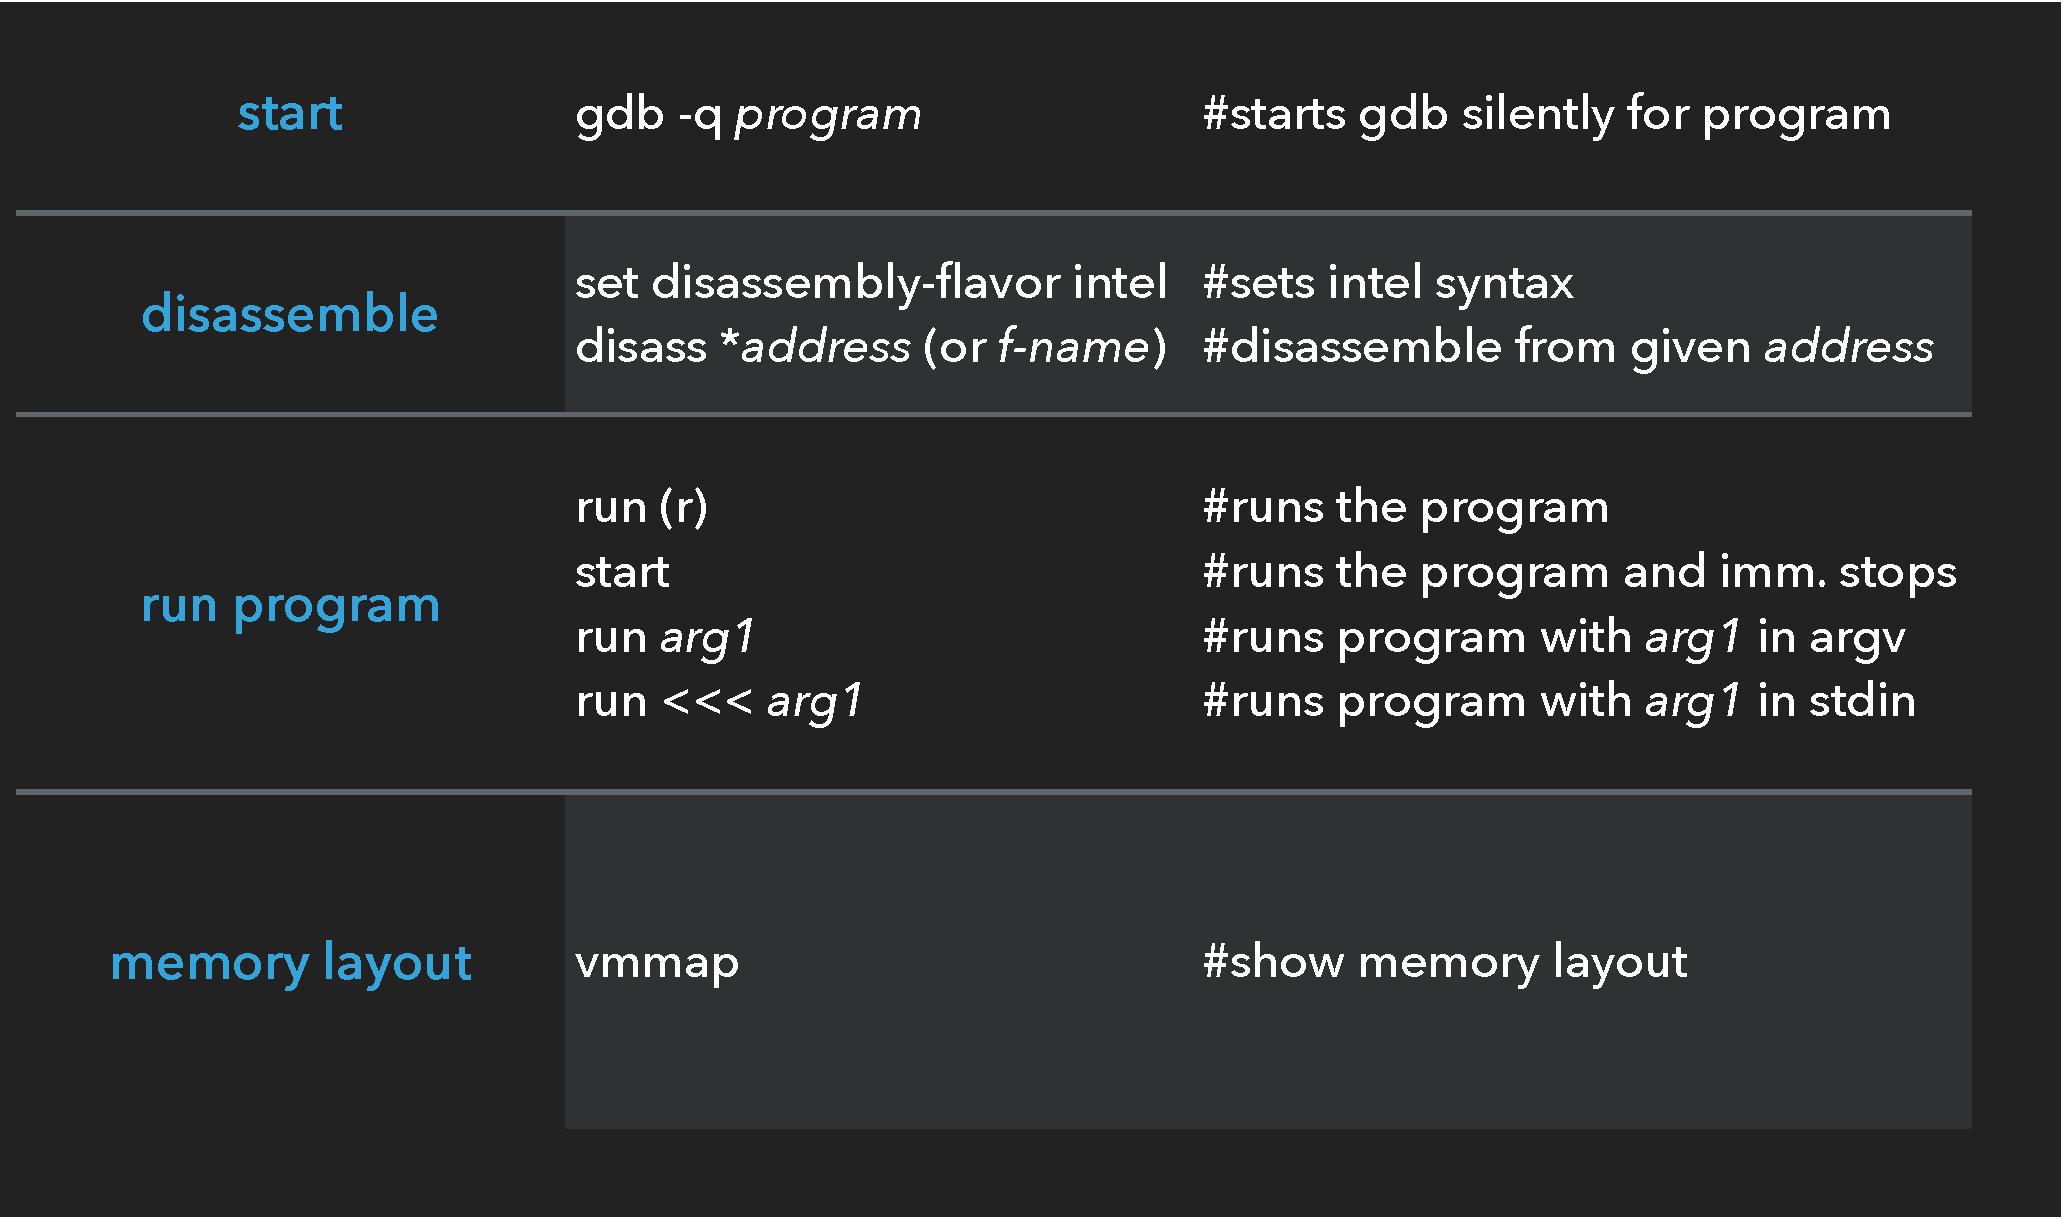
\includegraphics[width=\paperwidth]{./images/gdb_2.pdf}
\end{frame}

\begin{frame}
  \frametitle{GDB - How to Survive \footnote{CTRL + D to Exit}}
  \hspace*{-11mm}
  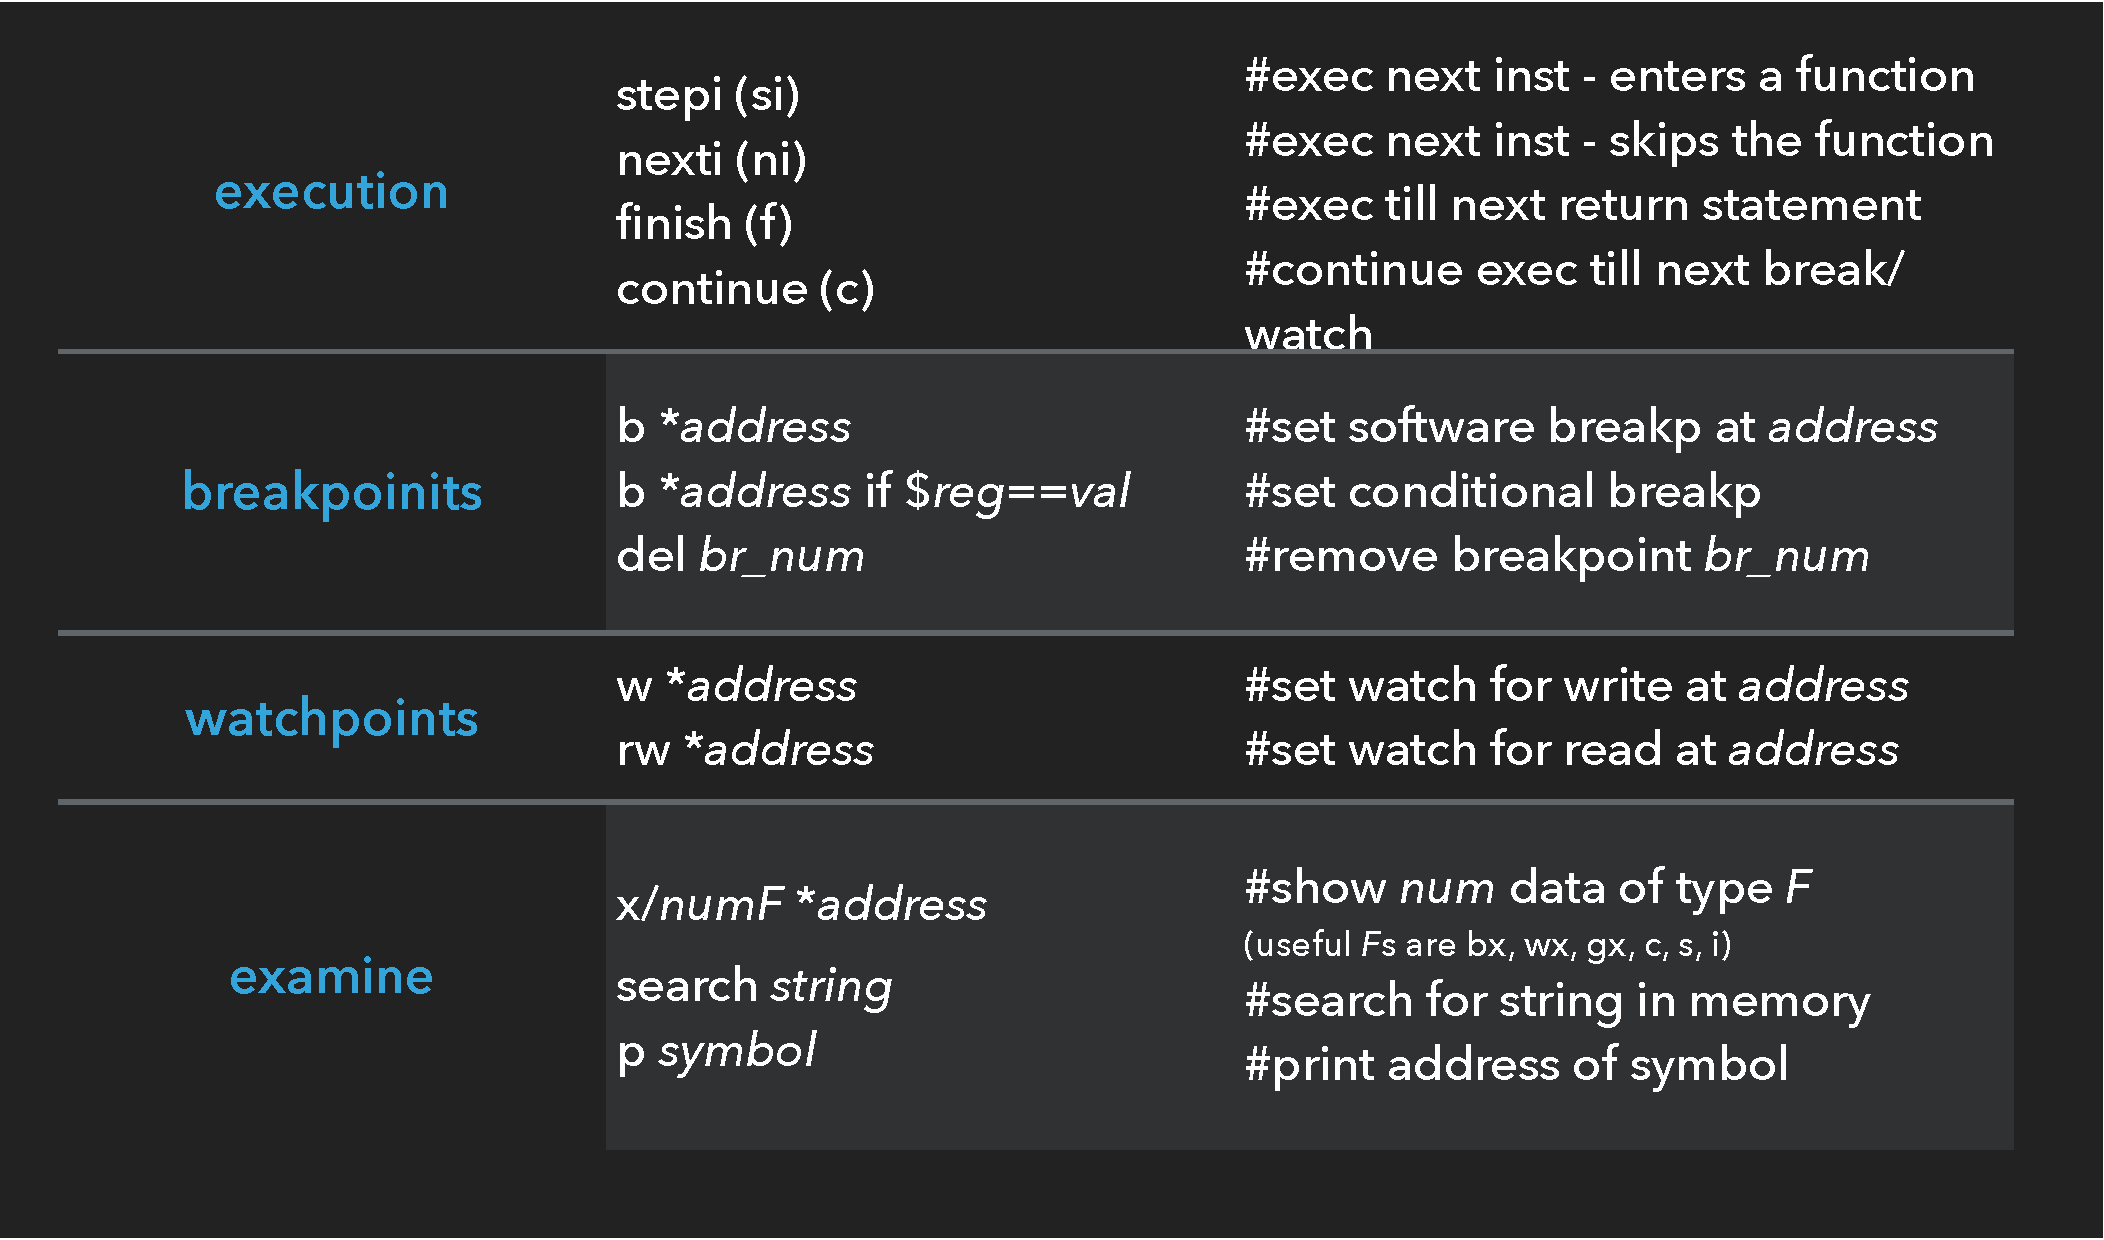
\includegraphics[width=\paperwidth]{./images/gdb_3.pdf}
\end{frame}


\begin{frame}{strace}
	\begin{itemize}
		\item Intercepts and records system calls and signals
		\item Dumps to standard error name, argument and return value of each system call
	\end{itemize}

	\begin{block}{Useful options}
		\begin{itemize}
			\item {\tt -p <pid>} attach to existing process
			\item {\tt -f} trace child process
			\item {\tt -o <filename>} output to file
			\item {\tt -e <expr>} modifies which events to trace (see manpage)
		\end{itemize}
	\end{block}
\end{frame}

\begin{frame}{ltrace}
	\begin{itemize}
		\item Intercepts and records dynamic library calls
		\item Similar to strace, but at a different layer
	\end{itemize}
\end{frame}

\begin{frame}[standout]
    Questions?
\end{frame}

\end{document}

%%% Local Variables:
%%% mode: latex
%%% TeX-master: t
%%% End:
